%
% File: chap01.tex
% Author: Victor F. Brena-Medina
% Description: Introduction chapter where the biology goes.
%
\let\textcircled=\pgftextcircled
\chapter{Related Work}
\label{chap2}

\initial{D}ue to the large potential practical values in many domains and the big technical challenges, video analysis has become a very hot research topic in both the academic and industrial communities in recent years. Since related works of interaction video analysis, such as \cite{patron2010} \cite{Gemeren2015} \cite{narayan2014} \cite{choi2012}, are relatively scarce compared to those in closely related areas, like action video analysis \cite{Ji2013} \cite{Ng2015} \cite{Tran2015} \cite{alex2008} \cite{grepory2010} \cite{karpathy2014} \cite{simonyan2014}, we will introduce both the architectures used in interaction and action video analysis related works in Section \ref{2_1}. The general architecture of a video recognizer is usually comprised of a feature descriptor and a classifier. The video feature description research can be mainly divided in two directions: hand-crafted feature descriptors and learning based feature descriptors. We will introduce these two types separately in Section \ref{2_2} and \ref{2_3} respectively. Another very important factor that determines the performance of the video analysis is the training datasets. Without a rich and nicely annotated training dataset, it is hard to get a decent performance even for the best-built algorithm. So, we will introduce popular publicly available action and interaction video datasets in Section \ref{2_4}.

%=======
\section{Architectures of Interaction video analysis related works}
\label{2_1}
Choi et al. \cite{choi2012} introduce a hierarchical network that recognizes the collective activity performed by a group of people. The hierarchical model is illustrated in Figure \ref{fig:hierA} (b). \(O_i\) and \(O_j\) are the features of each individual in the video, and \(O_c\) is the crowd context feature which represents the overall information of the video. \(A\) is the atomic action of each individual, \(I\) is the interaction between two individuals and \(C\) is the collective activity of the group of people. For example, the collective activity \("gathering"\), illustrated in Figure \ref{fig:hierA} (a), is characterized as a collection of interactions (such as \("approaching"\)) between individuals. Each interaction is described as pairs of atomic activities (for example \("facing-right"\) and \("facing-left"\)). Each atomic activity is associated with a spatial-temporal trajectory. \cite{choi2012} use HOG to represent the appearance features and use bag of video words (BoV \cite{bov}) to represent the spatial-temporal features.
\begin{figure}
	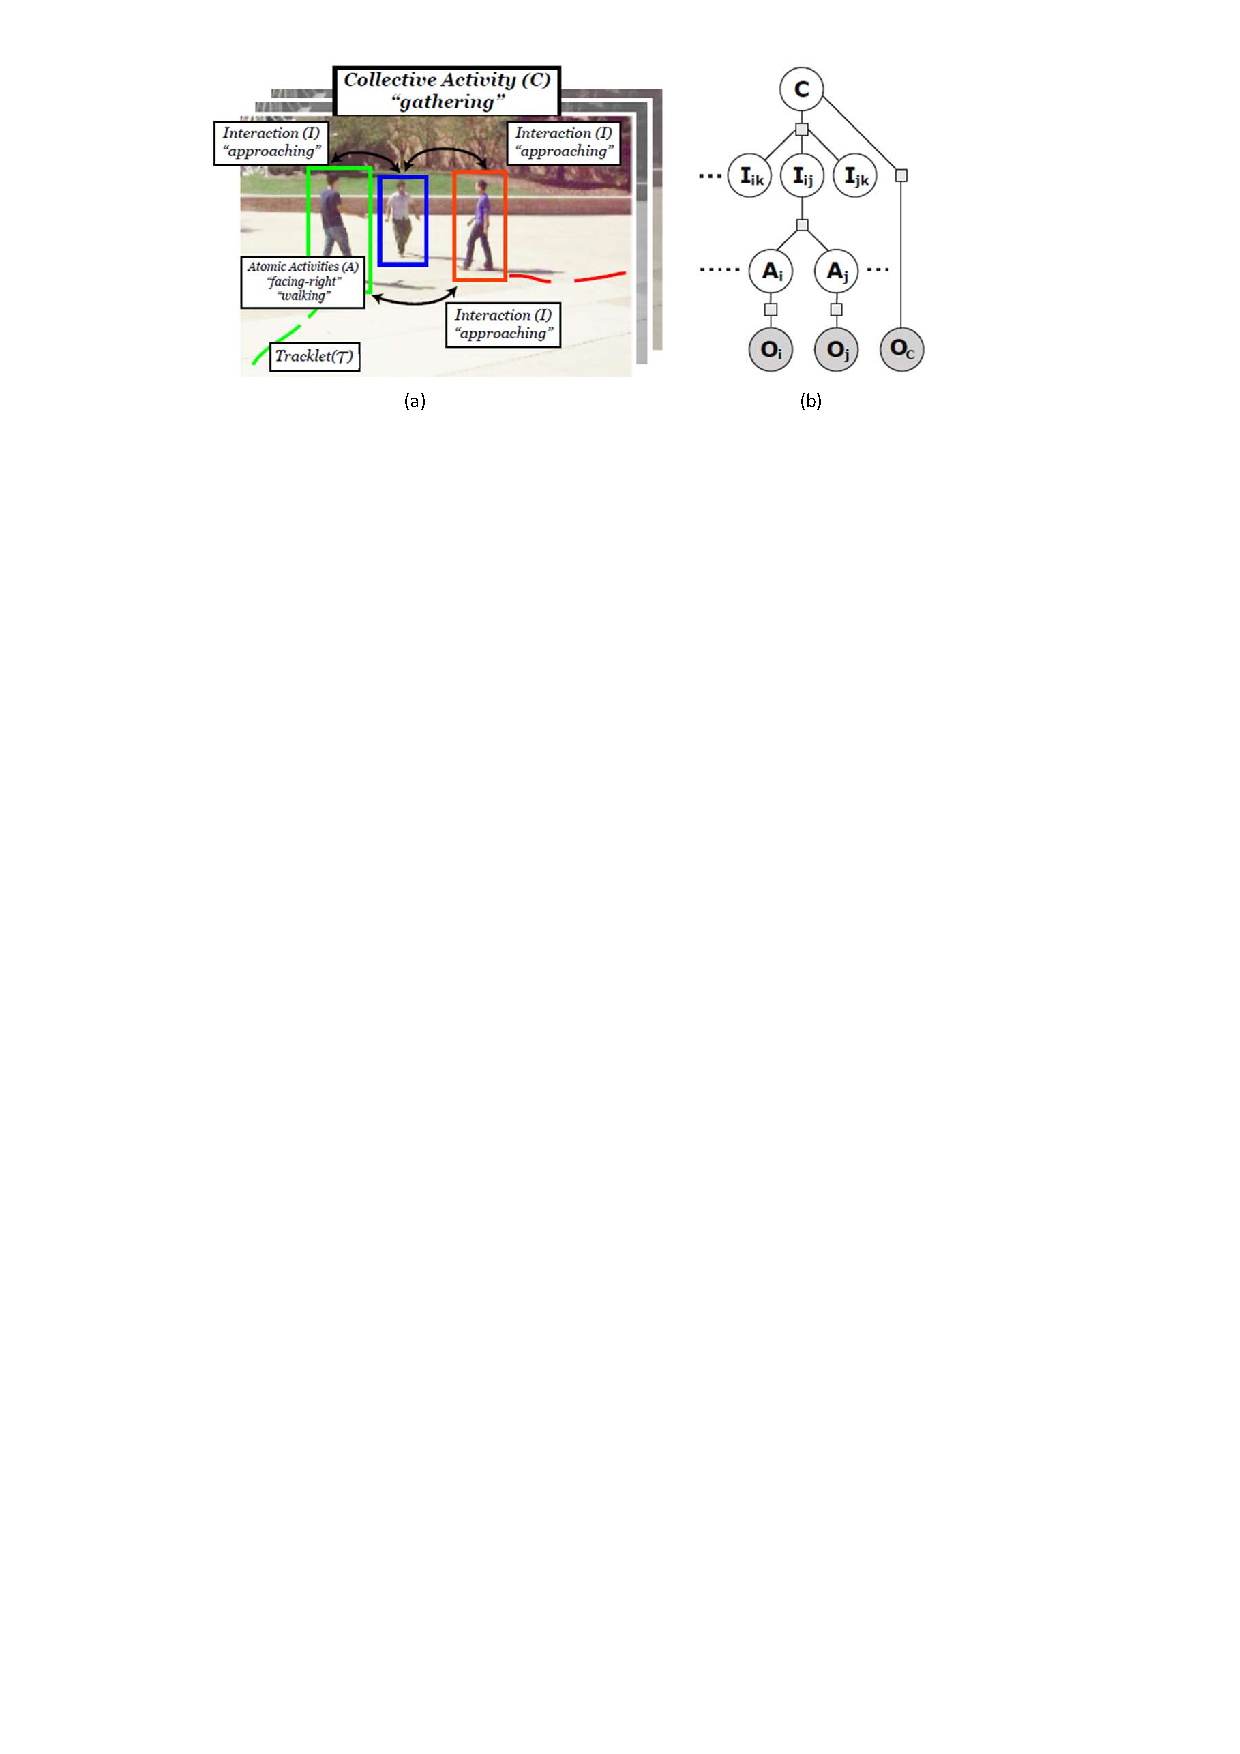
\includegraphics[trim=2cm 22.5cm 0cm 1cm]{figs/hier.pdf}
	\caption{The hierarchical activity recognition model and an example. Reprinted from \cite{choi2012}.}
	\label{fig:hierA}
\end{figure}
\par 
Compared with the work of Choi et al. which uses a hierarchical model to recognize group activities, Gemeren et al. \cite{Gemeren2015} extract the interaction features from the local body parts of the interacting people and focus on those parts of the videos that characterize the interaction. This is helpful in distinguishing between the interactions that only have  very slight differences. HOG (appearance) and HOF (movement) are combined as feature descriptors in this work.
\par
Patron-Perez et al.'s work \cite{patron2010} is similar to \cite{Gemeren2015}. Patron-Perez et al. detect and track each person's upper body in the interaction video and crop the tracklet to generate a person-centered descriptor with HOG and HOF. Besides, the head orientation is also taken into account in the feature descriptor because the head orientation is also an important cue for the interaction video analysis.
\par
There are also some methods that use a bag of the local features in order to describe the features of interaction, like the work of Yimeng et al. \cite{yimeng} and Yu et al. \cite{yu}. Yimeng et al. propose the concept of spatio-temporal phrase which is a combination of the local features in a certain spatial and temporal structure including their order and relative positions, then the video is represented by a bag of spatio-temporal phrases. Yu et al. propose the use of a set of attributes and the pair-wise co-occurrence relationship of two attributes to describe the videos. An attribute is a binary representation of a body part, such as that 'the torso is still'. A co-occurrence relationship of two attributes is a binary representation of the association between the two attributes. For example, the co-occurrence relationships between the attributes "torso bending" and "still leg" in the activity "bow".

\section{Hand-crafted Feature Descriptor}
\label{2_2}

The scale-invariant feature transform (SIFT \cite{lowe1999} \cite{lowe2004})  and the histogram of oriented gradients (HOG \cite{hog}) feature descriptors achieve great success and are widely applied in the image content analysis. 
\par 
SIFT is a local feature describing algorithm which detects the interest points in an image and computes the gradients for each interest point in order to construct the features of an image. The SIFT algorithm adopts the difference of Gaussian (DoG) algorithm to detect the interest points by constructing an image pyramid with several scales and blurring images with several different Gaussian filters in each scale. The interest points are those points that have maximum values compared with their neighbor pixels in the image pyramid. Thus, those points with edges and corners which represent the main feature of an object are most likely to be found as interest points. Because the interest points are detected in different scales, the  SIFT feature descriptor is scale invariant. Gradient computing is applied to the interest point centered blocks for each interest point. The computed histogram of gradient features are rotated to the main orientation for each interest point. Thus, it is rotation invariant. And finally, the features are normalized in order to further eliminate the effect of different lighting.
\par 
For the HOG algorithm, the image is divided into several small cells. The histograms of gradient ( orientation and magnitude) are computed for each cell. This is because the appearance and shape of an object can be nicely described by the gradient. The HOG feature descriptor is somewhat transform invariant because the features are computed in local cells, and because the features are normalized over the sliding overlap blocks which contain several cells in a single block so it is lighting invariant.
\par
Though SIFT and HOG can efficiently describe appearance and shape features in images, but they can not be directly used for video analysis tasks, because they not only require appearance and shape description but also motion description. Thus, they are also extended to 3D-SIFT\cite{grepory2010} \cite{paul2007} and 3D-HOG\cite{alex2008} in order to describe the video features. Among all current hand-crafted feature descriptors, the improved Dense Trajectories(iDT)\cite{wang2012}\cite{wang2013} have been shown to perform the best on a variety of datasets. 

\subsection{3D-SIFT Feature Descriptor}
\label{2_2_1}
Compared with 2D-SIFT \cite{lowe1999} \cite{lowe2004} which only considers \(x\) and \(y\) dimensions, 3D-SIFT \cite{grepory2010} \cite{paul2007} takes another dimension, in this case, \(time(t)\), into consideration because the motion information contained in time dimension is an essential cue for video analysis. There are two steps involved in the constructing of the SIFT feature descriptor. The first step is the localization of the key points and the second step is the calculation of the sub-histograms for each key point. The method of key points localization in the 3D-SIFT is the same as that in the 2D-SIFT. The main differences between 2D-SIFT and 3D-SIFT is the calculation of the sub-histogram for each key point.
\par 
The 2D gradient magnitude and orientation for each pixel are calculated in \(x\) and \(y\) dimensions, while 3D-SIFT calculates gradients in three dimensions \(x\), \(y\) and \(t\). Thus, the motion information along the time dimension is also well presented by the sub-histogram of 3D gradients.
  
\begin{figure}
	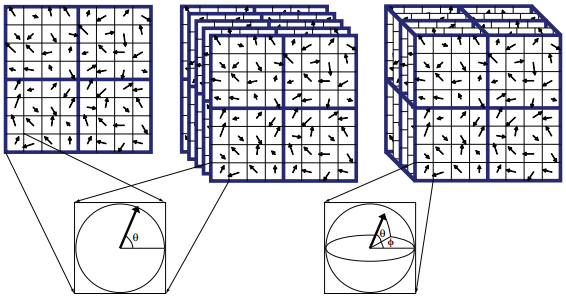
\includegraphics[width=\linewidth]{figs/3D_SIFT.png}
	\caption{The SIFT descriptor. The left image shows the 2D SIFT descriptor. The center image shows how multiple 2D SIFT descriptor could be used on a video without modification to the original method. The right image shows the 3D SIFT descriptor with its 3D sub-volumes, each sub-volume is accumulated into its own sub-histogram. These histograms are what makes up the final descriptor. Reprinted from \cite{grepory2010}.}
	\label{fig:3DSIFT}
\end{figure}
\par 
The 3D-SIFT feature descriptor is illustrated in Figure \ref{fig:3DSIFT}. After getting the sub-histogram, the orientation of each key point could be fixed. In 3D-SIFT, the dominant orientation of the key point could be represented by\(\) \(\theta\) and \(\phi\). To keep the orientation invariant, all neighbourhoods of each key point are rotated to the dominant orientation. 3D-SIFT also inherits the method of key points detection and histogram normalization from 2D-SIFT. Thus, it is also scale and lighting invariant. 


\subsection{3D-HOG Feature descriptor}
\label{2_2_2}
2D-HOG is widely used for the purpose of object detection in static images. 2D-HOG calculates the gradients for each pixel and accumulates them as the histograms of orientated gradient over cells. Klaser et al. extend it to 3D-HOG \cite{alex2008}. In Klaser's work, the main difference between 2D and 3D HOG is the calculation of the gradient. In 2D-HOG, only two dimensions \(x\) and \(y\) are taken into account, the cell is a square. While in 3D-HOG, additional time dimension \(t\) is taken into consideration, so the cell is a cube. The blocks which are used to contrast-normalization also transform from a 2D square to a 3D cube. The overview of the descriptor computation is illustrated in Figure \ref{fig:3DHOG}.
\begin{figure}
	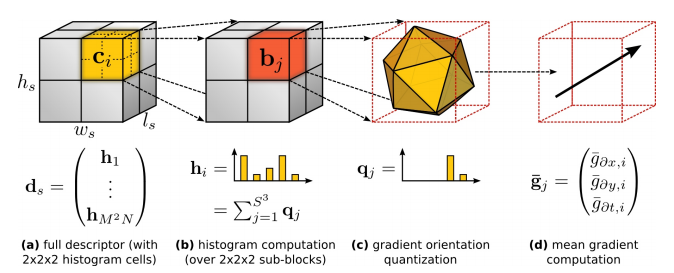
\includegraphics[width=\linewidth]{figs/3D_HOG.png}
	\caption{ Overview of 3D-HOG descriptor computation; (a) the support region around a point
		of interest is divided into a grid of gradient orientation histograms; (b) each histogram is
		computed over a grid of mean gradients; (c) each gradient orientation is quantized using
		regular polyhedrons; (d) each mean gradient is computed using integral videos. Reprinted from \cite{alex2008}.}
	\label{fig:3DHOG}
\end{figure}
\par 

For similar reasons found in 3D-SIFT, 3D-HOG calculates the gradients in both spatial and temporal dimensions, so, the motion information contained in the time dimension can be nicely represented by the 3D-gradients. 

\subsection{Improved Dense Trajectories feature descriptor}
\label{2_2_3}

The Improved Dense Trajectory (iDT) is a very successful algorithm used for video action recognition among all hand-crafted feature descriptors which was proposed by Wang et al. \cite{wang2012} \cite{wang2013}.  Wang et al. \cite{wang2012} introduce the Dense Trajectory (DT) algorithm and they improve the DT algorithm by eliminating background optical flow trajectory caused by the camera motion in \cite{wang2013}.
\par
The overview of the DT feature descriptor is illustrated in Figure \ref{fig:DT}, which includes dense sampling, key points tracking and features description. The video is firstly extended into several different spatial scales in order to keep this feature descriptor scale invariant.
\par 
Feature points are densely sampled on a grid spaced by \(W\) pixels and the sampling is carried out on each spatial scale separately. Since it is hard to track feature points in homogeneous areas, Wang et el. remove those points which have very small eigenvalues of the auto-correlation matrix. 
\par 
Feature points are then separately tracked on each spatial scale. Given a point \(P_t = (x_t,y_t)\) in frame \(I_t\), its tracked position in the \(I_{t+1}\) frame  is calculated by the position in \(I_t\) frame and the components of optical flow computed  w.r.t. \(I_t\) and \(I_{t+1}\). Due to the fact that it is unstable to track a feature point for a long time, all the feature points are re-sampled every \(L\) frames. Then, for every feature point, the trajectory feature vector is \((P_t,P_{t+1},P_{t+2}....,P_{t+L-1})\). The trajectory feature vector contains the motion information of the feature points thus it can represent motion information for the videos. 
\par 
Since just the trajectory features are not enough to describe all the video features, Wang et al. introduce another three feature descriptors: Histograms of Orientated Gradient (HOG \cite{hog}), Histograms of Optical Flow (HOF \cite{hof} and Motion Boundary Histograms (MBH \cite{hof}). The HOG feature descriptor is similar to 3D-HOG but it is calculated along the trajectory. The HOF features represent the optical flow (movements) of objects in videos and the MBH features are based on the derivatives of optical flow which is a simple and effective way to suppress the camera motion. 3D-HOG can well represent both the appearance/shape and the motion information for objects in videos. The combination of HOF and MBH can further improve the performance of video analysis as they represent zero-order (HOF) and first-order (MBH) motion information. All of these three feature descriptors are calculated in a \(N*N*L\) spatial-temporal volume around the feature point along the trajectory, see the right image in Figure \ref{fig:DT}. The spatial-temporal volume is sliced into smaller \(n\sigma * n\sigma * n\tau \) spatial-temporal cells. \(N= 32, n\sigma = 2, n\tau = 3 \) in the work of Wang et al. The histogram of HOG, HOF and MBH are calculated over all the pixels contained in each cell.

\begin{figure}
	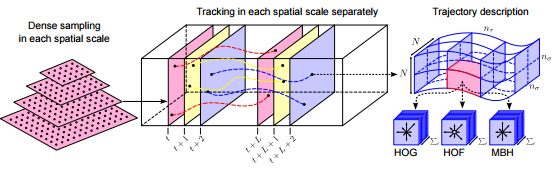
\includegraphics[width=\linewidth]{figs/DT.png}
	\caption{Illustration of DT algorithm to extract and characterize dense trajectories. Left: Feature points
		are densely sampled on a grid for each spatial scale. Middle: Tracking is carried out in the corresponding
		spatial scale for L frames by median filtering in a dense optical flow field. Right: The trajectory shape
		is represented by relative point coordinates, and the descriptors (HOG, HOF, MBH) are computed along
		the trajectory in a \(N * N\) pixels neighbourhood, which is divided into \(n\sigma * n\sigma * n\tau \) cells. Reprinted from \cite{wang2012}.}
	\label{fig:DT}
\end{figure}
 
\par 
The work of iDT \cite{wang2013} improves the DT algorithm mainly by eliminating the camera motion. In the DT algorithm, due to the camera motion, many trajectories in the background are found. But those trajectories of background are useless for action recognition and usually giving confusing results. By assuming that the difference between 2 consecutive frames is small, the iDT algorithm assumes that the frame \(I_{t+1}\) can be calculated from frame \(I_t\) and a transform matrix \(H\), that \(I_{t+1} = I_t * H \).  Then, we can calculate \(Iwarp_{t+1} = H^{-1} * I_{t+1}\), where \(Iwarp_{t+1}\) is the frame \(I_{t+1}\) after eliminating the camera motion. Since the transformation matrix \(H\) is calculated over the whole image \(I_t\) and \(I_{t+1}\) which include both background and interest human. So, the large movement of the human body in consecutive frames will largely affect the accuracy of matrix \(H \). Wang et al. use the human detection technique to detect the human body in all images and mask these areas to get a more accurate transform matrix \(H\) and use this matrix to eliminate the useless trajectory of the background and the human body that is caused by camera motion.

\section{Deep Learning Based Feature Descriptor}
\label{2_3}

Though hand-crafted feature descriptors achieve very nice performance in terms of image and video content analysis, they are all based on pre-defined rules to extract features. Thus, they usually ignore the potential cues for video analysis which are not implemented by the feature designer. A deep learning based feature descriptor has complex parameters and flexible structure. A well trained deep learning feature descriptor can represent similar features represented by hand-crafted feature descriptor. For example, the Convolutional Neural Network (CNN or ConvNet \cite{cnn}) can learn about edges in lower layers which is similar to HOG. Furthermore, a well trained deep learning feature descriptor has the potential abilities to represent some features which are hard for hand-crafted features descriptors which means that  learning feature descriptors are more general than hand-crafted feature descriptors.  Due to the significant development of data science, deep learning based feature descriptors, especially CNN,  show powerful ability for feature representation and have achieved state-of-the-art performance in image classification/recognition \cite{kaiming}.
\par 
The Convolutional Neural Network is one type of deep artificial neural network in which the connectivity patterns between its neurons is inspired by the organization of animal's visual cortex. The architecture of one of the very first ConvNets, the LeNet5 by Yann LeCun et al. \cite{cnn}, is illustrated in Figure \ref{fig:cnn}. A typical ConvNet includes three main parts: the convolutional layers, the pooling/subsampling layers and the fully connected layers. The convolutional layer extracts features from input image by applying convolution. The convolution can be understood as a feature filter applied over the input image. We can perform operations such as edge detection by just setting different filter parameters. So, one filter (convolutional kernel) can extract one type of features. The more filters, the more features that can be represented by the ConvNet. An intuitive example of convolution is illustrated in Figure \ref{fig:conv}. The pooling/subsampling layer reduces the dimensionality of each feature map but retain the most important information. There are different types of pooling: Max pooling which takes the largest element in a \(n \times n\) window; and Average pooling which takes the average value of all elements in the window. The pooling operation can simplify the features and thus has the following advantages: 1). Making the network smaller and more manageable; 2). Reducing the number of parameters and computation, therefore controlling over-fitting; 3). Making the network invariant to small transformations, distortions, etc. The fully connected layer is a traditional multi layer perceptron in which every neuron in the previous layer is connected to every neuron in the next layer. The output of the convolutional and pooling layers represents high-level features of input images while the fully connected layers use these features to classify the input images into various classes.  

\begin{figure}
	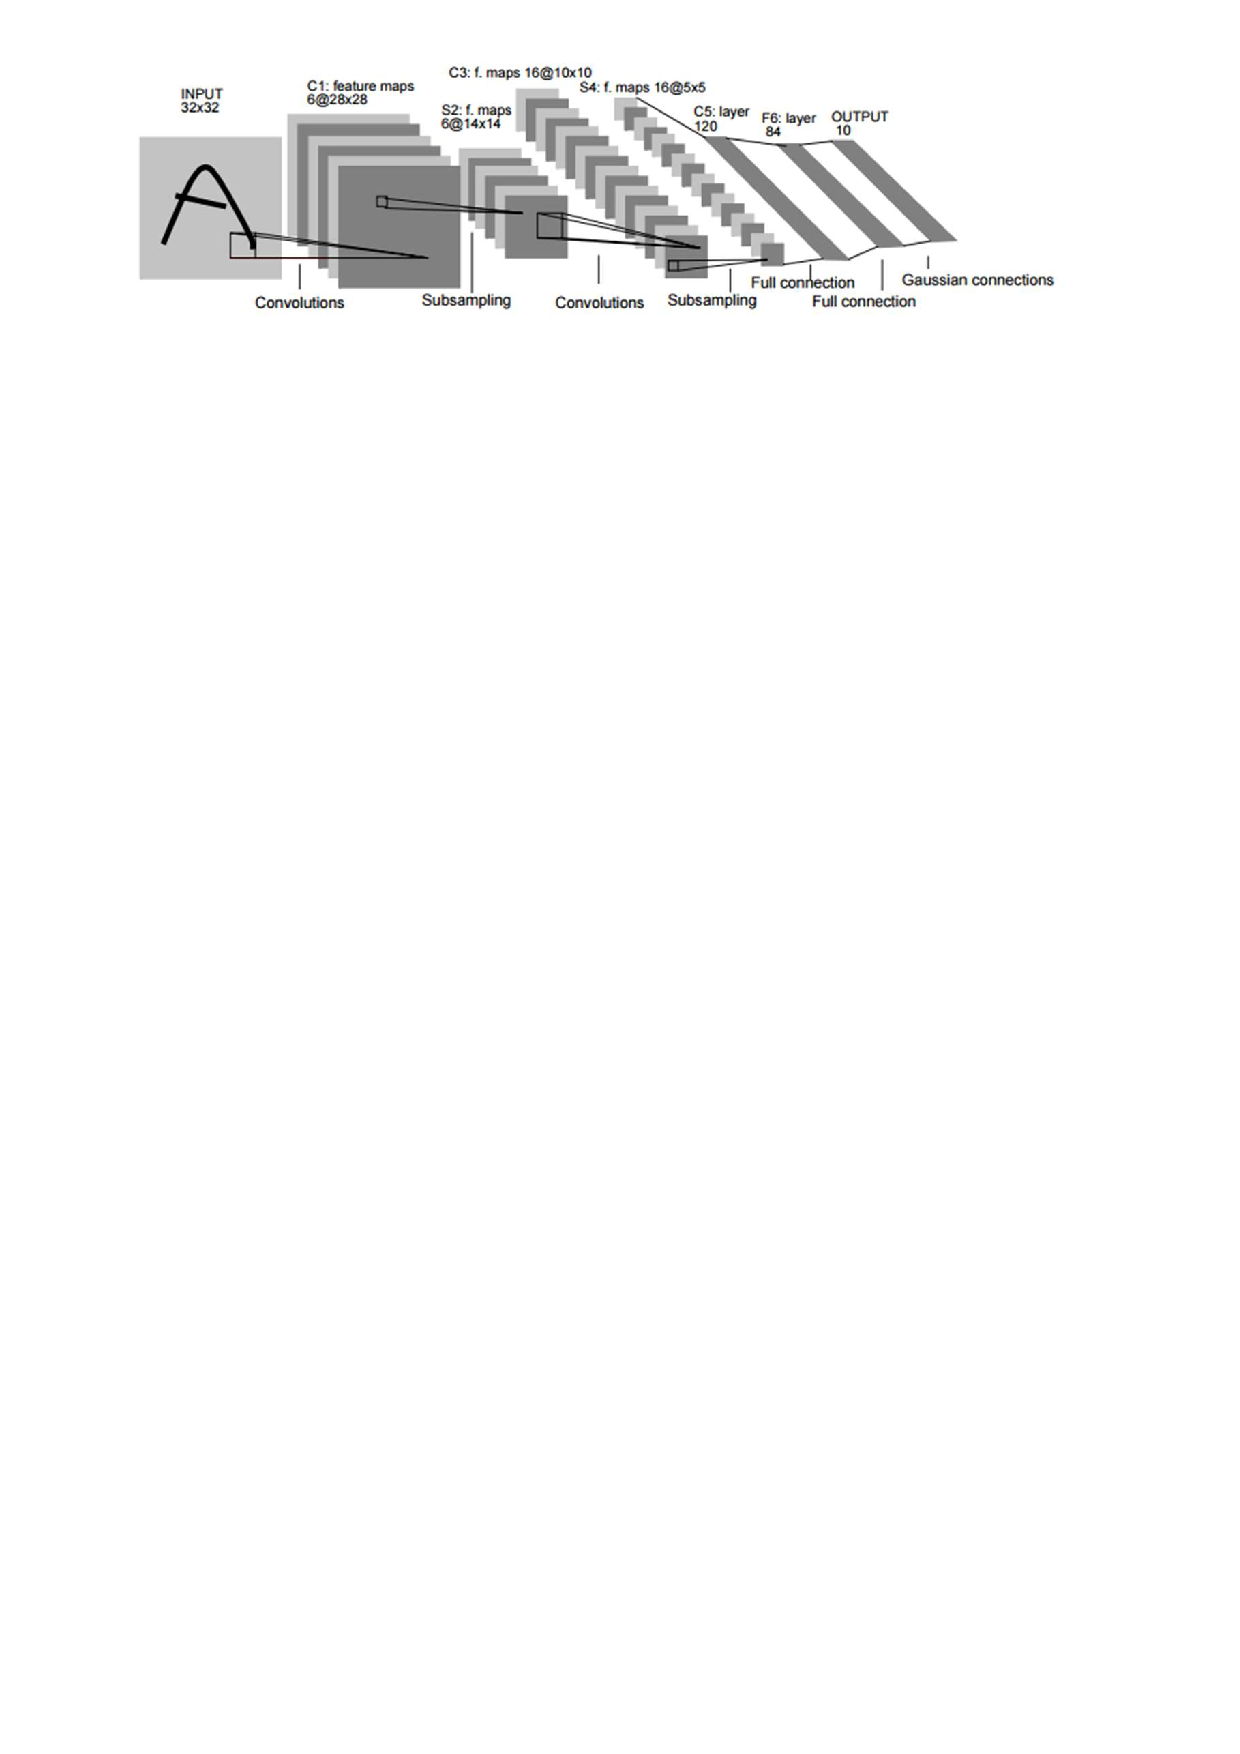
\includegraphics[trim=2cm 23cm 0cm 1cm]{figs/cnn.pdf}
	\caption{The architecture of a CNN example: LeNet5. Reprinted from \cite{cnn}.}
	\label{fig:cnn}
\end{figure}

\begin{figure}
	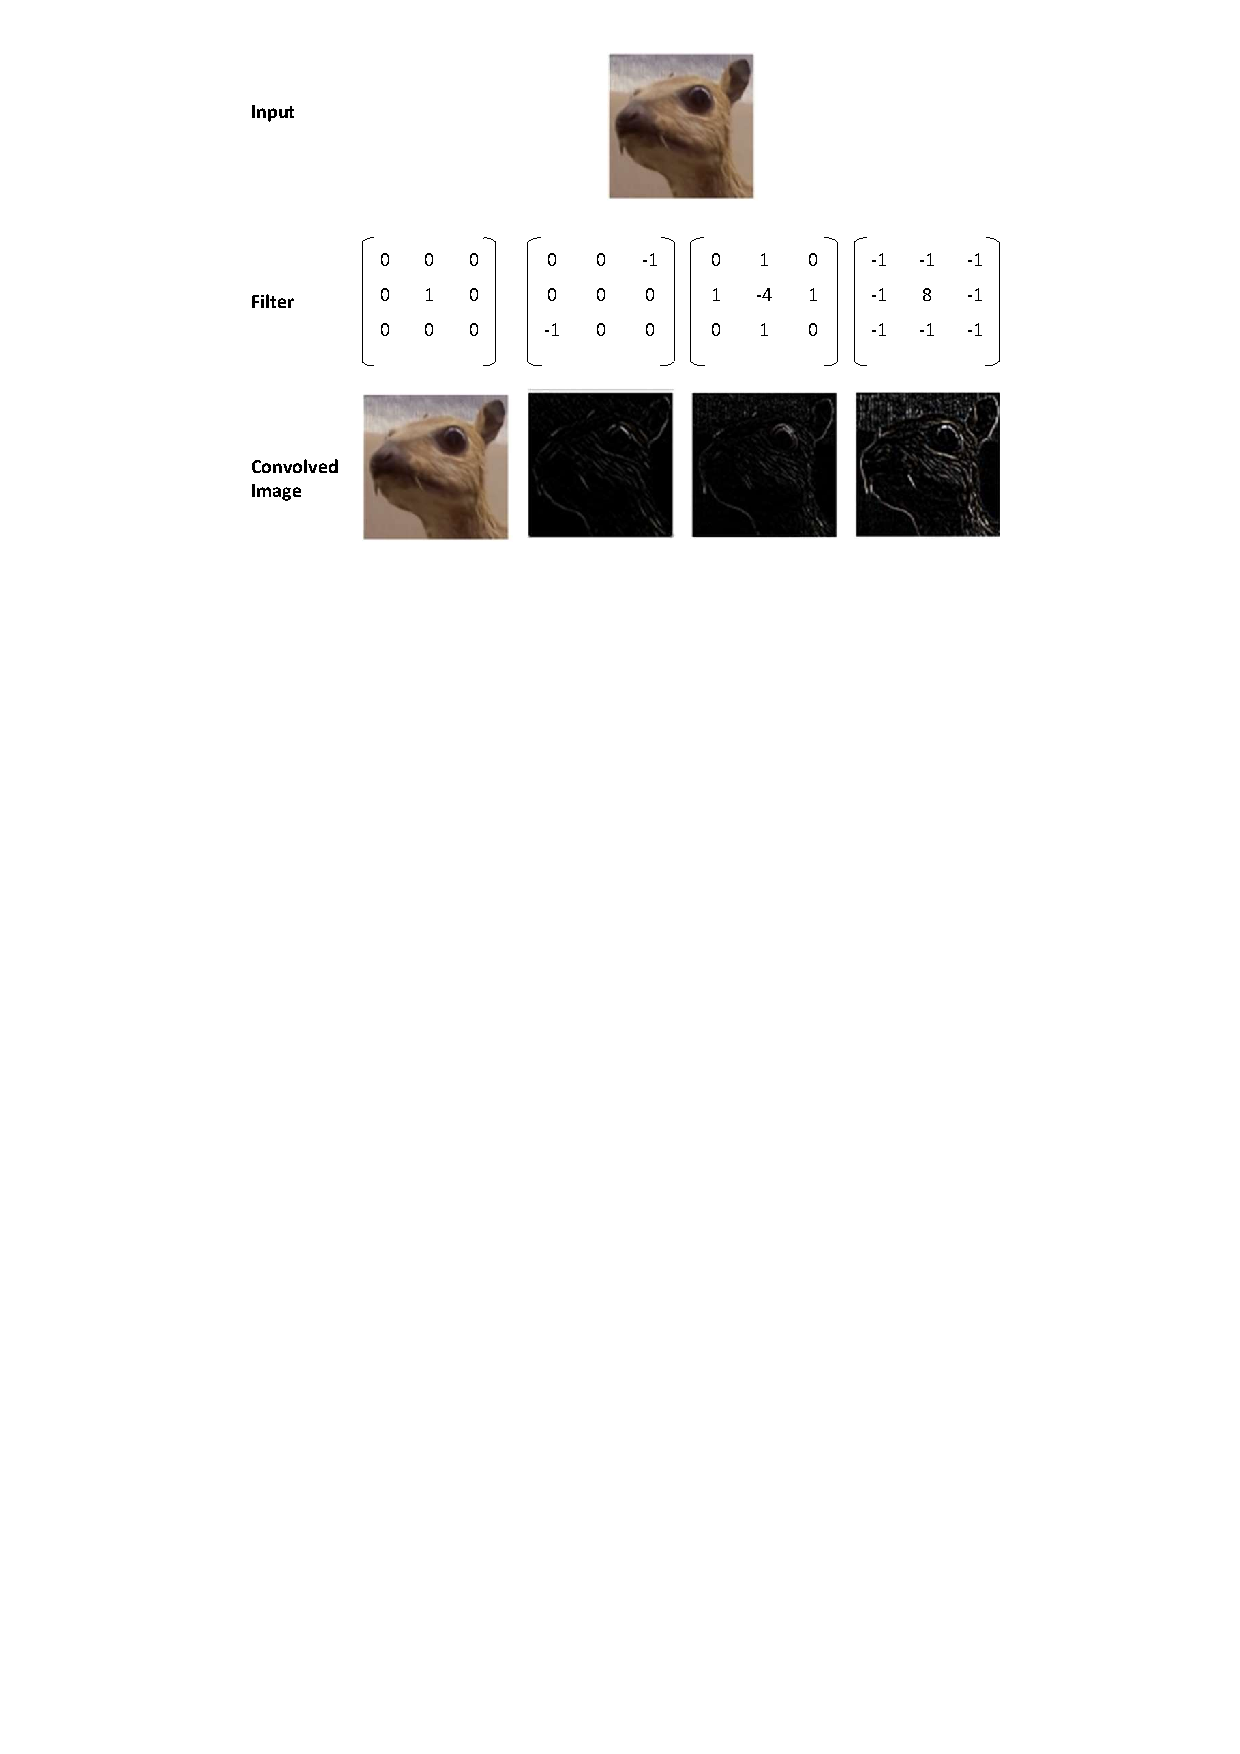
\includegraphics[trim=2cm 20cm 0cm 1cm]{figs/conv.pdf}
	\caption{The intuitive illustration of convolution over image.}
	\label{fig:conv}
\end{figure}
 
\par
There is related work \cite{ning2005} in the earlier stages which just simply applies CNN and treats the videos as a set of single frames, then averages the results over all frames as the overall result. The performance of such method is not very satisfying since it doesn't take the important temporal information into consideration and there may be many irrelevant frames in the video will confuse the result. In recent years, many new related works have been proposed in order to solve these problems, like the Spatial-Temporal CNN\cite{karpathy2014}, Two-Stream ConvNet\cite{simonyan2014}, and 3D Convolutional Networks(3D-ConvNet) \cite{3dcnn_1} \cite{Ji2013} \cite{Tran2015}.  

\subsection{Spatial-Temporal CNNs feature descriptor}
\label{2_3_1}

Since spatial information represents the appearance and the temporal information represents motion, they are both essential for video analysis. Karpathy et al. suggested a spatial-temporal CNN in their work\cite{karpathy2014}. They studied several approaches to extend the connectivity of CNNs to time domain in order to make use of the spatial-temporal information contained in videos, including late fusion, early fusion and slow fusion. The architectures of fusion CNNs are illustrated in Figure \ref{fig:STCNNs}. 
\par 
Single frame architecture is used as a baseline in the work \cite{karpathy2014}. It is a standard CNN framework and is similar to the ImageNet challenge winning model \cite{kriz2012} just with a different input image resolution. The architecture of the single frame network is illustrated in Figure \ref{fig:STCNNs} (a).
\par 
The late fusion model, illustrated in Figure \ref{fig:STCNNs} (b), places two separate single frame networks that share the network parameters. The inputs of the two networks are two streams which have a distance of 15 frames. The two networks are merged in the first fully connected layer. Neither single network alone can detect any motion, but the first full connected layer can compute global motion characteristics by comparing the outputs of the two networks. 
\par 
The early fusion model, illustrated in Figure \ref{fig:STCNNs} (c), is similar to the single frame model except that the input is consecutive \(T\) frames instead of a single frame. \(T\) was set to \(10\) in the work \cite{karpathy2014}. The early and direct connectivity to pixel data allows the network to precisely detect direction and speed of the local motion.
\par 
The slow fusion model, illustrated in Figure \ref{fig:STCNNs} (d),  combines the early and late fusion model. This model slowly fuses the temporal information throughout the network so that higher layers get access to progressively more global information in both the spatial and temporal dimensions. 

\begin{figure}
	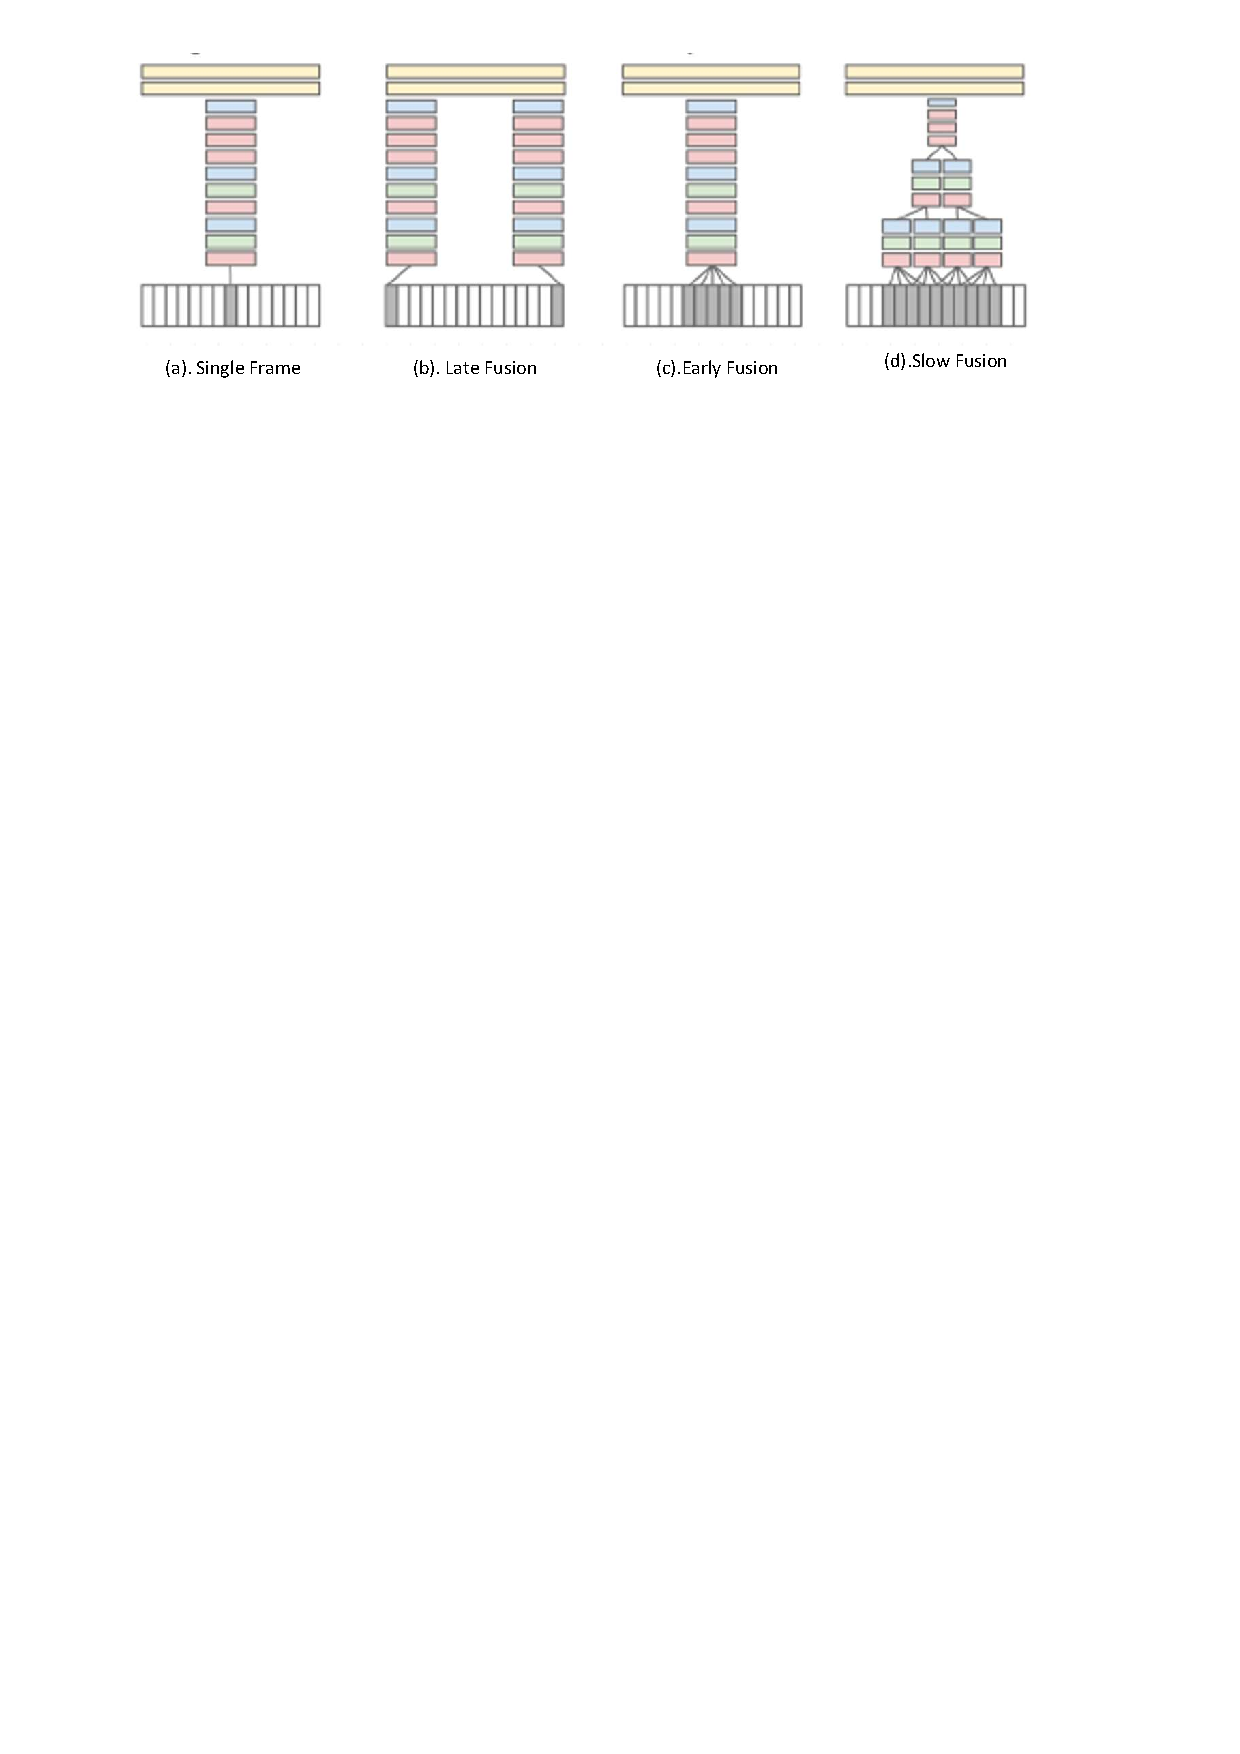
\includegraphics[trim=2cm 23cm 0cm 1cm]{figs/STCNNs.pdf}
	\caption{Explored approaches for fusing information over
		temporal dimension through the network. Red, green and
		blue boxes indicate convolutional, normalization and pooling
		layers respectively. In the Slow Fusion model, the depicted
		columns share parameters. Reprinted from \cite{karpathy2014}.}
	\label{fig:STCNNs}
\end{figure}

\subsection{Two-Stream ConvNet feature descriptor}
\label{2_3_2}
The Two-Stream ConvNet proposed by Simonyan et al. \cite{simonyan2014} is another extension of ConvNet for action recognition in video data. The Two-Stream ConvNet introduces a different architecture with the Spatial-Temporal CNNs \cite{karpathy2014} based on two separate recognition streams (spatial and temporal), which are combined through late fusion. The spatial stream learns the appearance features from the still video frames while the temporal stream learns the motion features in the form of the dense optical flow of input videos. So, the combination of the spatial and temporal streams can represent both the appearance/shape and motion for the input videos. The architecture of Two Stream ConvNet is illustrated in Figure \ref{fig:tsconvnet_1}.

\begin{figure}
	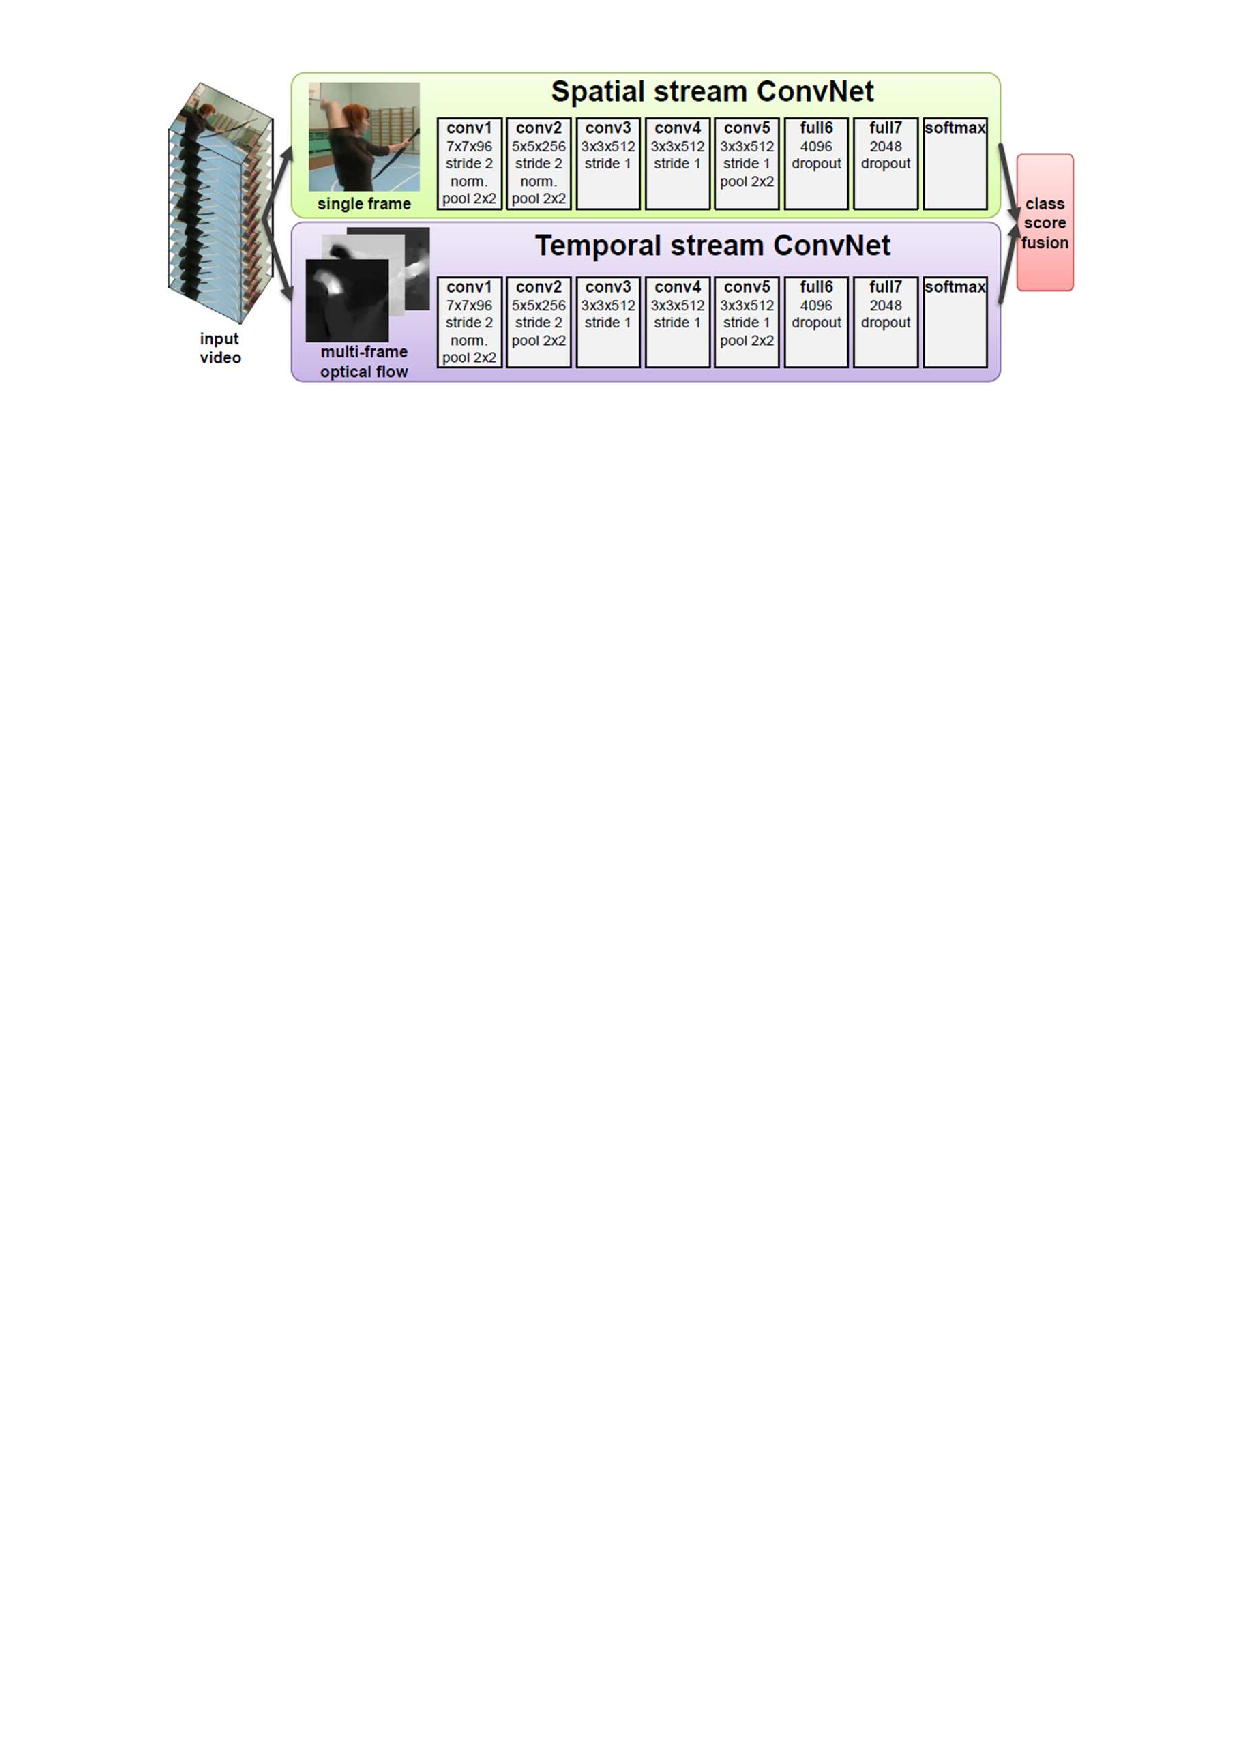
\includegraphics[trim=2cm 23cm 0cm 1cm]{figs/tsconvnet.pdf}
	\caption{The architecture of Two Stream ConvNet. Reprinted from \cite{simonyan2014}.}
	\label{fig:tsconvnet_1}
\end{figure}
   

\subsection{3D ConvNet feature descriptor}
\label{2_3_3}
3D ConvNet was first proposed by Ji et al. \cite{Ji2013} with human body segmented video volumes as input and Tran et al. \cite{Tran2015} improved it by making it accept full raw video volumes as input without any pre-processing. The main difference between 2D ConvNets and 3D ConvNets is that the convolution and pooling are applied in three dimensions (\(x\),\(y\),\(time\)) instead of two (\(x\),\(y\)). As illustrated in Figure \ref{fig:3DConv}, 2D convolution applied on a single image or a video volume (multiple frames as multiple channels) all result in an image, while 3D Convolution on a video volume results in another video volume. So, the video temporal information is lost after applying 2D convolution, while the 3D convolution preserves both the spatial and temporal information. 
\par 
The network architecture used in \cite{Tran2015} annotated as C3D is illustrated in Figure \ref{fig:3DConvNet}. The input of the network is a 16 frames video volume. Videos with frame number larger than 16 will be split into several 16 frames video clips with an overlap of 8 frames for each video clip.  Features are calculated separately for all video clips, and the features of video clips which belong to the same video are simply averaged to generate the finally features of the video. 
\par
The Figure \ref{fig:3DConvNetV} illustrates what the 3D ConvNet learns by using the de-convolution method explained in \cite{zeiler2014}. In both examples, the features first focus on the appearance and gradually track the motion over the rest of the frames. 

\begin{figure}
	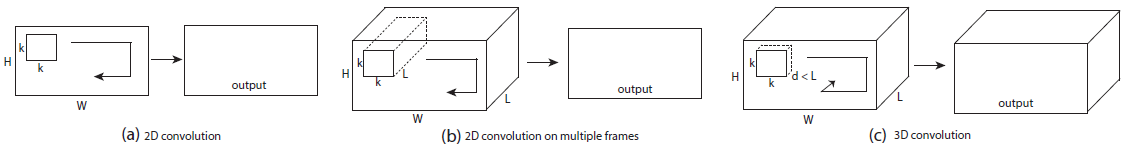
\includegraphics[width=\linewidth]{figs/3DConv.png}
	\caption{2D and 3D convolution operations. a) Applying 2D convolution on an image results in an image. b) Applying 2D convolution
		on a video volume (multiple frames as multiple channels) also results in an image. c) Applying 3D convolution on a video volume results
		in another volume, preserving temporal information of the input signal. Reprinted from \cite{Tran2015}.}
	\label{fig:3DConv}
\end{figure}

\begin{figure}
	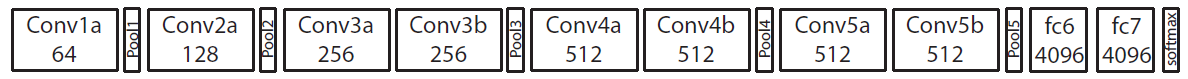
\includegraphics[width=\linewidth]{figs/3DConvNet.png}
	\caption{The architecture of C3D. C3D has 8 convolution, 5 max-pooling, and 2 full connected layers, followed by a softmax output layer. All 3D convolution kernels are \(3 \times 3 \times 3\) with stride 1 in both spatial and temporal dimensions. Number of filters are denoted in each box. The 3D pooling layers are denoted from pool1 to pool5. All pooling kernels are \(2 \times 2 \times 2\) except for pool1 is \(1 \times 2 \times 2\). Each fully connected layer has 4096 output units. Reprinted from \cite{Tran2015}.}
	\label{fig:3DConvNet}
\end{figure}

\begin{figure}
	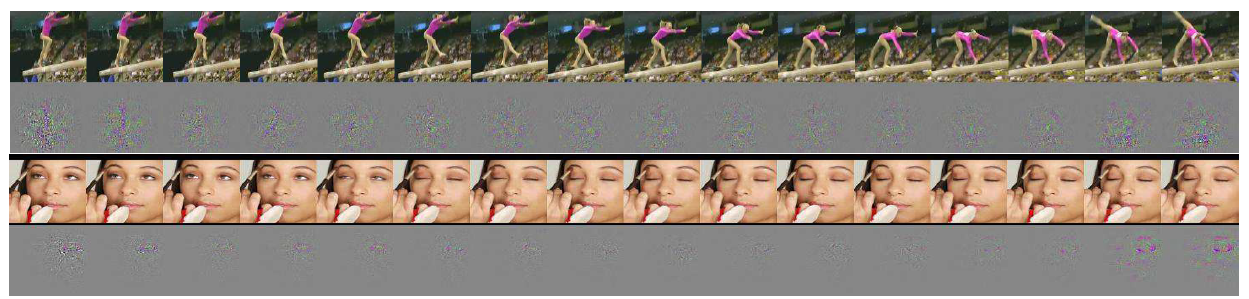
\includegraphics[width=\linewidth]{figs/3DConvNetV.png}
	\caption{Visualization of C3D model. Interestingly, C3D captures appearance for the first few frames but thereafter only attends to salient motion. Reprinted from \cite{Tran2015}.}
	\label{fig:3DConvNetV}
\end{figure}

\section{Datasets}
\label{2_4}

Training dataset is one of the key factors needed to train a high-performance feature descriptor. At the same time, published and widely used datasets can be helpful for comparing between different approaches. After the publication of the KTH \cite{kth} dataset which contains 6 action classes and 600 videos (2391 sequences) in 2004, more and more human activity datasets have been published. In recent years, the development of datasets has the following characteristics:
\begin{enumerate}
	\item More action classes. KTH has 6 classes, UCF101 \cite{ucf101} has 101 action classes and ASLAN \cite{aslan} has 432 classes.
	\item More training and testing samples. KTH has 192 videos for training and 216 videos for testing, while ActivityNet 200 \cite{activitynet200} has 10024 videos for training and 5044 videos for testing.
	\item The video scenes become more and more complex. The videos of KTH are acted by very limited number of actors, while recent datasets are cut from realistic scenes, like youtube, cctv, BBC etc.
	\item More challenges in the video content; from fixed backgrounded without camera motion to  non-static camera, multi-viewpoints, more complex backgrounds; from single person action to  human-human interaction, human-object interaction, etc.    
\end{enumerate}  

\subsection{List of human activity video datasets}
Part of the widely used action and interaction video datasets are illustrated in Table \ref{table:action_datasets} and Table \ref{table:interaction_datasets}, respectively.
\begin{table}
	\caption{List of human action video datasets}
	\begin{center}
		\begin{tabular}{| p{2.5cm} | p{1.5cm} | p{4cm} | p{3cm} | p{4cm} |}
			\hline
			Dataset & Classes & Videos & Annotations & Properties \\ \hline \hline
			% *********************************************************************
			% KTH 
			% *********************************************************************
			KTH\cite{kth} 
			& % classes
			6 action classes 
			& % videos 
			\vspace{-5mm}
			\begin{myitemize}
				\item Training : 192
				\item Validation: 192
				\item Testing: 216
				\item Resolution: \(160 \times 120\) @ 25fps
			\end{myitemize}
            & % anotations
			\vspace{-5mm}
			\begin{myitemize}
				\item Action labels
				\item Temporal segments
			\end{myitemize}
	    	& %properties
	    	\vspace{-5mm}
	    	\begin{myitemize}
	    		\item Static camera
	    		\item Simple background
	    		\item Acted by 25 subjects, 6 actions and 4 scenarios
	    	\end{myitemize}
    		\\ \hline 
	    	
	    	% **********************************************************************
	    	% Hollywood2
	    	% **********************************************************************
	    	Hollywood2\cite{marszalek09}
	    	& % classes
	    	12 action classes and 10 scene classes
	    	& % videos 
	    	For actions:
	    	\vspace{-3mm}
	    	\begin{myitemize}
	    		\item Training : 823
	    		\item Testing: 884	
	    	\end{myitemize}
    		For scenarios:
    		\vspace{-3mm}
    		\begin{myitemize}
    			\item Training : 570
    			\item Testing: 582	
    		\end{myitemize}
    		Resolution: \(400-300 \times 300-200\)
	    	& % anotations
	    	\vspace{-5mm}
	    	\begin{myitemize}
	    		\item Action labels
	    		\item Scene labels
	    	\end{myitemize}
	    	& %properties
	    	\vspace{-5mm}
	    	\begin{myitemize}
	    		\item Non-static camera
	    		\item Realistic scenarios from movies
	      	\end{myitemize}
	    	\\ \hline 


	    	% **********************************************************************
	    	% UCF101
	    	% **********************************************************************
	    	UCF101\cite{ucf101}
	    	& % classes
	    	5 types, 101 action classes
	    	& % videos 
	    	\vspace{-5mm}
	    	\begin{myitemize}
	    		\item Training : 9537
	    		\item Testing: 3783
	    		\item Resolution: \(400-300 \times 300-200\)	
	    	\end{myitemize}
	    	
	    	& % anotations
	    	\vspace{-5mm}
	    	\begin{myitemize}
	    		\item Action labels
	    	\end{myitemize}
	    	& %properties
	    	\vspace{-5mm}
	    	\begin{myitemize}
	    		\item Realistic scenarios from YouTube
	    		\item Large variations in camera motion, object appearance and pose, object scale, viewpoints, cluttered background, illumination conditions, etc.
	    	\end{myitemize}
	    	\\ \hline
	    	
	    	
	    	% **********************************************************************
	    	% ActivityNet
	    	% **********************************************************************
	    	ActivityNet 200\cite{activitynet200}
	    	& % classes
	    	200 action classes
	    	& % videos 
	    	\vspace{-5mm}
	    	\begin{myitemize}
	    		\item Training : 10024
	    		\item Validation: 4926
	    		\item Testing: 5044
	    	\end{myitemize}
	    	
	    	& % anotations
	    	\vspace{-5mm}
	    	\begin{myitemize}
	    		\item Action labels
	    		\item Temporal segments
	    		\item Hierarchy activities relationship
	    	\end{myitemize}
	    	& %properties
	    	\vspace{-5mm}
	    	\begin{myitemize}
	    		\item Realistic scenarios
	    		\item Large variations in camera motion, object appearance and pose, object scale, viewpoints, cluttered background, illumination conditions, etc.
	    	\end{myitemize}
	    	\\ \hline
   	
		\end{tabular}
		\label{table:action_datasets}
	\end{center}
\end{table}

\begin{table}
	\caption{List of human interaction video datasets}
	\begin{center}
		\begin{tabular}{| p{2.5cm} | p{1.5cm} | p{4cm} | p{3cm} | p{3cm} |}
			\hline
			Dataset & Classes & Videos & Annotations & Properties \\ \hline \hline
			
			% **********************************************************************
			% UT-Interaction
			% **********************************************************************
			UT-Interaction\cite{ut2010}
			& % classes
			6 interaction classes
			& % videos 
			\vspace{-5mm}
			\begin{myitemize}
				\item 20 videos
				\item 2 sets, 10 for each set. Evaluated by leave one out cross validation.
				\item Resolution = \(720 \times 480\)
			\end{myitemize}
			
			& % anotations
			\vspace{-5mm}
			\begin{myitemize}
				\item Interaction labels
				\item Temporal segments
				\item Spatial segments
			\end{myitemize}
			& %properties
			\vspace{-5mm}
			\begin{myitemize}
				\item Two-person interaction
				\item Static camera
				\item Acted in different background
			\end{myitemize}
			\\ \hline
			
			% **********************************************************************
			% ShakeFive2
			% **********************************************************************
			ShakeFive2\cite{shakefive2}
			& % classes
			8 interaction classes
			& % videos 
			\vspace{-5mm}
			\begin{myitemize}
				\item 153 videos
				\item Resolution = \(1280 \times 720\)
			\end{myitemize}
			
			& % anotations
			\vspace{-5mm}
			\begin{myitemize}
				\item Interaction labels
				\item Joint position
				\item Temporal segments
			\end{myitemize}
			& %properties
			\vspace{-5mm}
			\begin{myitemize}
				\item Homogeneous background 
				\item Static camera
			\end{myitemize}
			\\ \hline
			
			% **********************************************************************
			% MMI
			% **********************************************************************
			Multi-modal \& Multi-view \& Interactive \cite{m2i_tju}
			& % classes
			9 interaction classes and 13 person-object interaction classes
			& % videos 
			\vspace{-5mm}
			\begin{myitemize}
				\item 1760 RGB videos
				\item 1760 depth videos
				\item Resolution = \(320 \times 240\)
			\end{myitemize}
			
			& % anotations
			\vspace{-5mm}
			\begin{myitemize}
				\item Interaction labels
				\item Joint position
				\item Foreground mask
			\end{myitemize}
			& %properties
			\vspace{-5mm}
			\begin{myitemize}
				\item Homogeneous background 
				\item Static camera
			\end{myitemize}
			\\ \hline
			
			
		\end{tabular}
		\label{table:interaction_datasets}
	\end{center}
\end{table}

\subsection{UT-Interaction dataset}
\label{ut-interaction}
We use UT-Interaction dataset \cite{ut2010} as the main target interaction dataset to train and evaluate our interaction classification and detection model. We first introduce the basic information of this dataset followed by some special challenges about it and the last for the evaluation methodology.
\subsubsection*{Introductions of the basic information of the UT-Interaction dataset}
The UT-Interaction dataset contains videos of continuously executions of 6 classes of human-human interactions, including hand shaking, hugging, kicking, pointing, punching and pushing, as shown in Figure \ref{fig:ut_6classes}.

\begin{figure}
	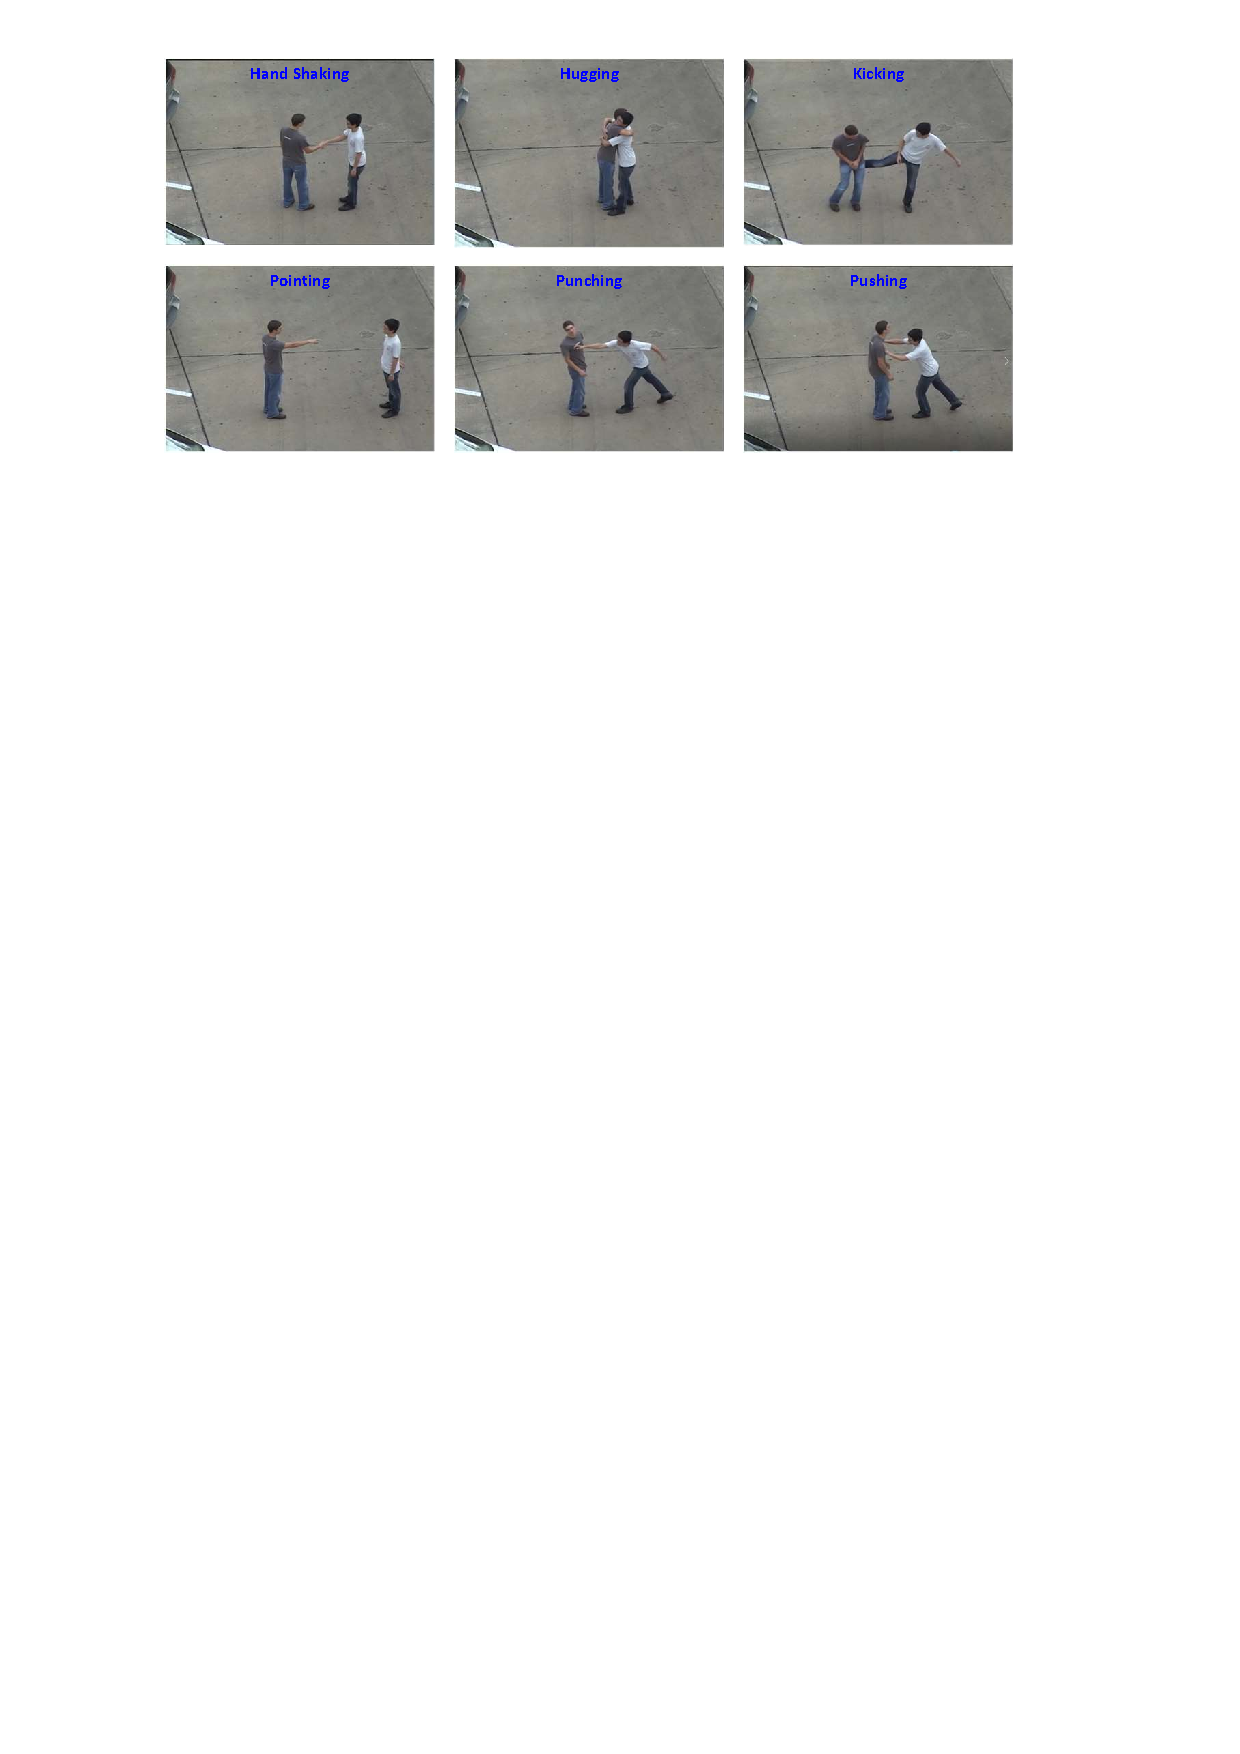
\includegraphics[trim=2cm 22cm 0cm 1cm]{figs/ut_6classes.pdf}
	\caption{The illustration of the 6 classes of  human-human interactions in the UT-Interaction dataset.}
	\label{fig:ut_6classes}
\end{figure}
 There are 20 video sequences whit about 1 minute lengths for each. Each video contains at least one execution per interaction, providing us 6 executions of human-human interactions per video on average. Several participants with more than 15 different clothing conditions appear in the videos. The videos are taken with the resolution of \(720 \times 480\), and the height of a person in the video is about 200 pixels. Ground truth labels of interaction are provided, including time intervals and bounding boxes. 
 \par 
 These 20 videos are divided into two sets. The set1 is composed of 10 video sequences taken on a paring lot. The videos of the set1 are taken with slight different zoom rate, and their backgrounds are mostly static with little camera jitter. While the set2 (the other 10 video sequences) are taken on a lawn in a windy day. The backgrounds are moving slightly, for example tree moving, and they contain more camera jitters. The illustrations of the different backgrounds between the two sets are shown in Figure \ref{fig:ut_2sets}.
 \begin{figure}
 	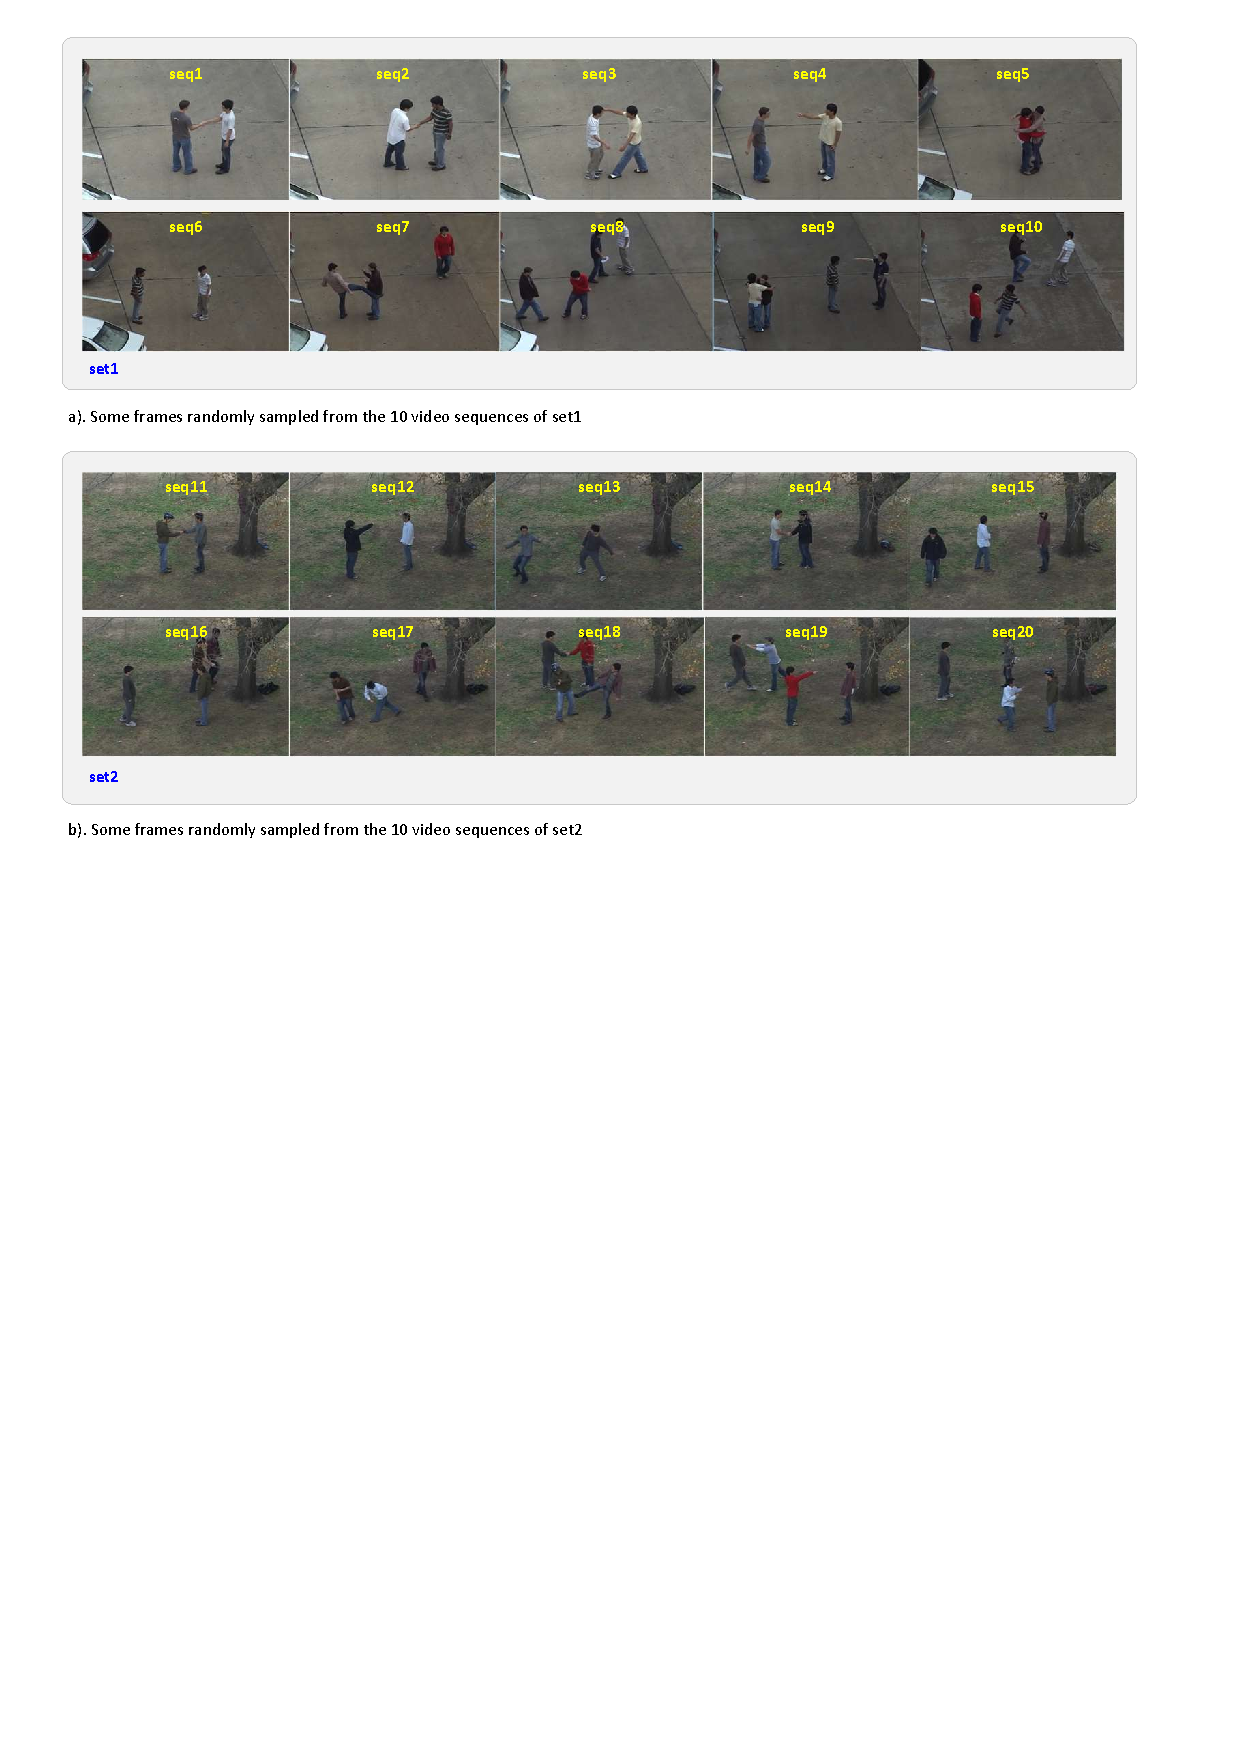
\includegraphics[trim=2cm 15.5cm 0cm 1cm]{figs/ut_2sets.pdf}
 	\caption{The illustration of the different backgrounds between the two sets}
 	\label{fig:ut_2sets}
 \end{figure}

\subsubsection*{The evaluation methodology}
We evaluate our models with two different experimental settings: classification and detection. 
\par 
For the \textquotesingle classification \textquotesingle \ task, the two sets of videos are evaluated separately. There are 120 video segments which are cropped based on the ground truth and each contains exactly one execution of one type of interaction. So, for each set, we have 60 segmented videos that will be used for the training and testing. The cropped video segments are illustrated in Figure.  10-fold leave-one-out cross validation is employed to evaluate the classification accuracy. That is, for each set, we leave one among 10 sequences for the testing and use the other 9 for the training. The performance is measured ten times and the average accuracy is used as the overall accuracy. 
\begin{equation*}
\text{Classification Accuracy} = \frac{\sum_{i=1}^{10} Accuracy_i }{10}
\end{equation*}
Where \(Accuracy_i\) is the classification accuracy of the \(ith\) sequence.
\begin{figure}
	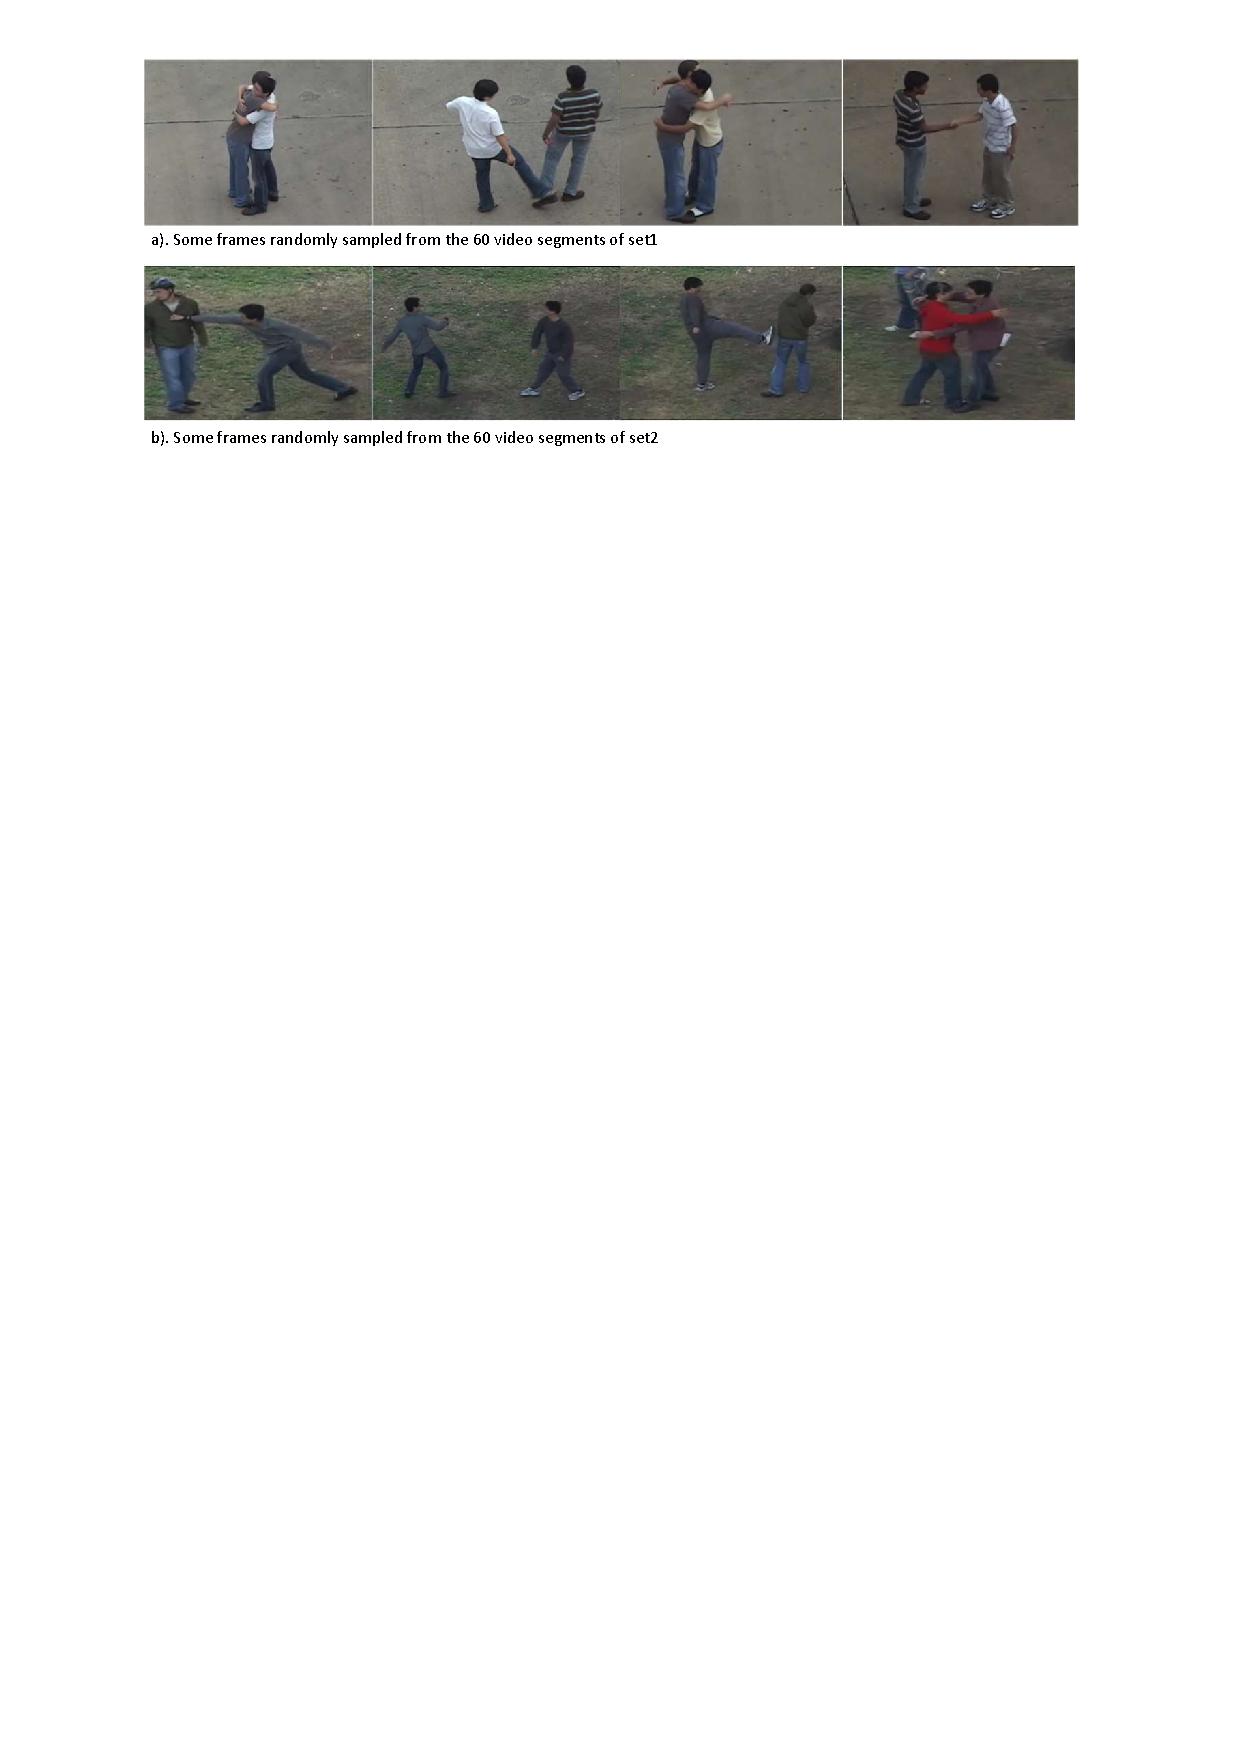
\includegraphics[trim=2cm 22cm 0cm 1cm]{figs/ut_segments.pdf}
	\caption{Some frames randomly sampled from the 120 segmented videos. }
	\label{fig:ut_segments}
\end{figure}
\par 
For the \textquotesingle detection\textquotesingle \ task, the interaction detection is measured to be correct if and only if the network correctly annotates an occurring interaction's time interval and spatial bounding box. If the detection overlaps the ground truth more than 50\% spatially and temporally, the detection is treated as a true positive. Otherwise, it is treated as a false positive.  i.e.
\begin{equation*}
\frac{\text{Detection} \cap \text{Ground Truth}}{\text{Detection} \cup \text{Ground Truth}} > 50\%
\end{equation*}
The \textquotesingle Detection \textquotesingle \ here is a 3D volume, its label, location and size are given by the output of the interaction detector. And  \textquotesingle Ground Truth \textquotesingle \ here is also a 3D volume which has the same class label with the \textquotesingle detection \textquotesingle. The location and size of the \textquotesingle Ground Truth \textquotesingle \ are provided by the ground truth table.  The illustration of \textquotesingle Detection \textquotesingle \ and \textquotesingle Ground Truth \textquotesingle \ is shown in Figure \ref{fig:ut_det}.
\begin{figure}
	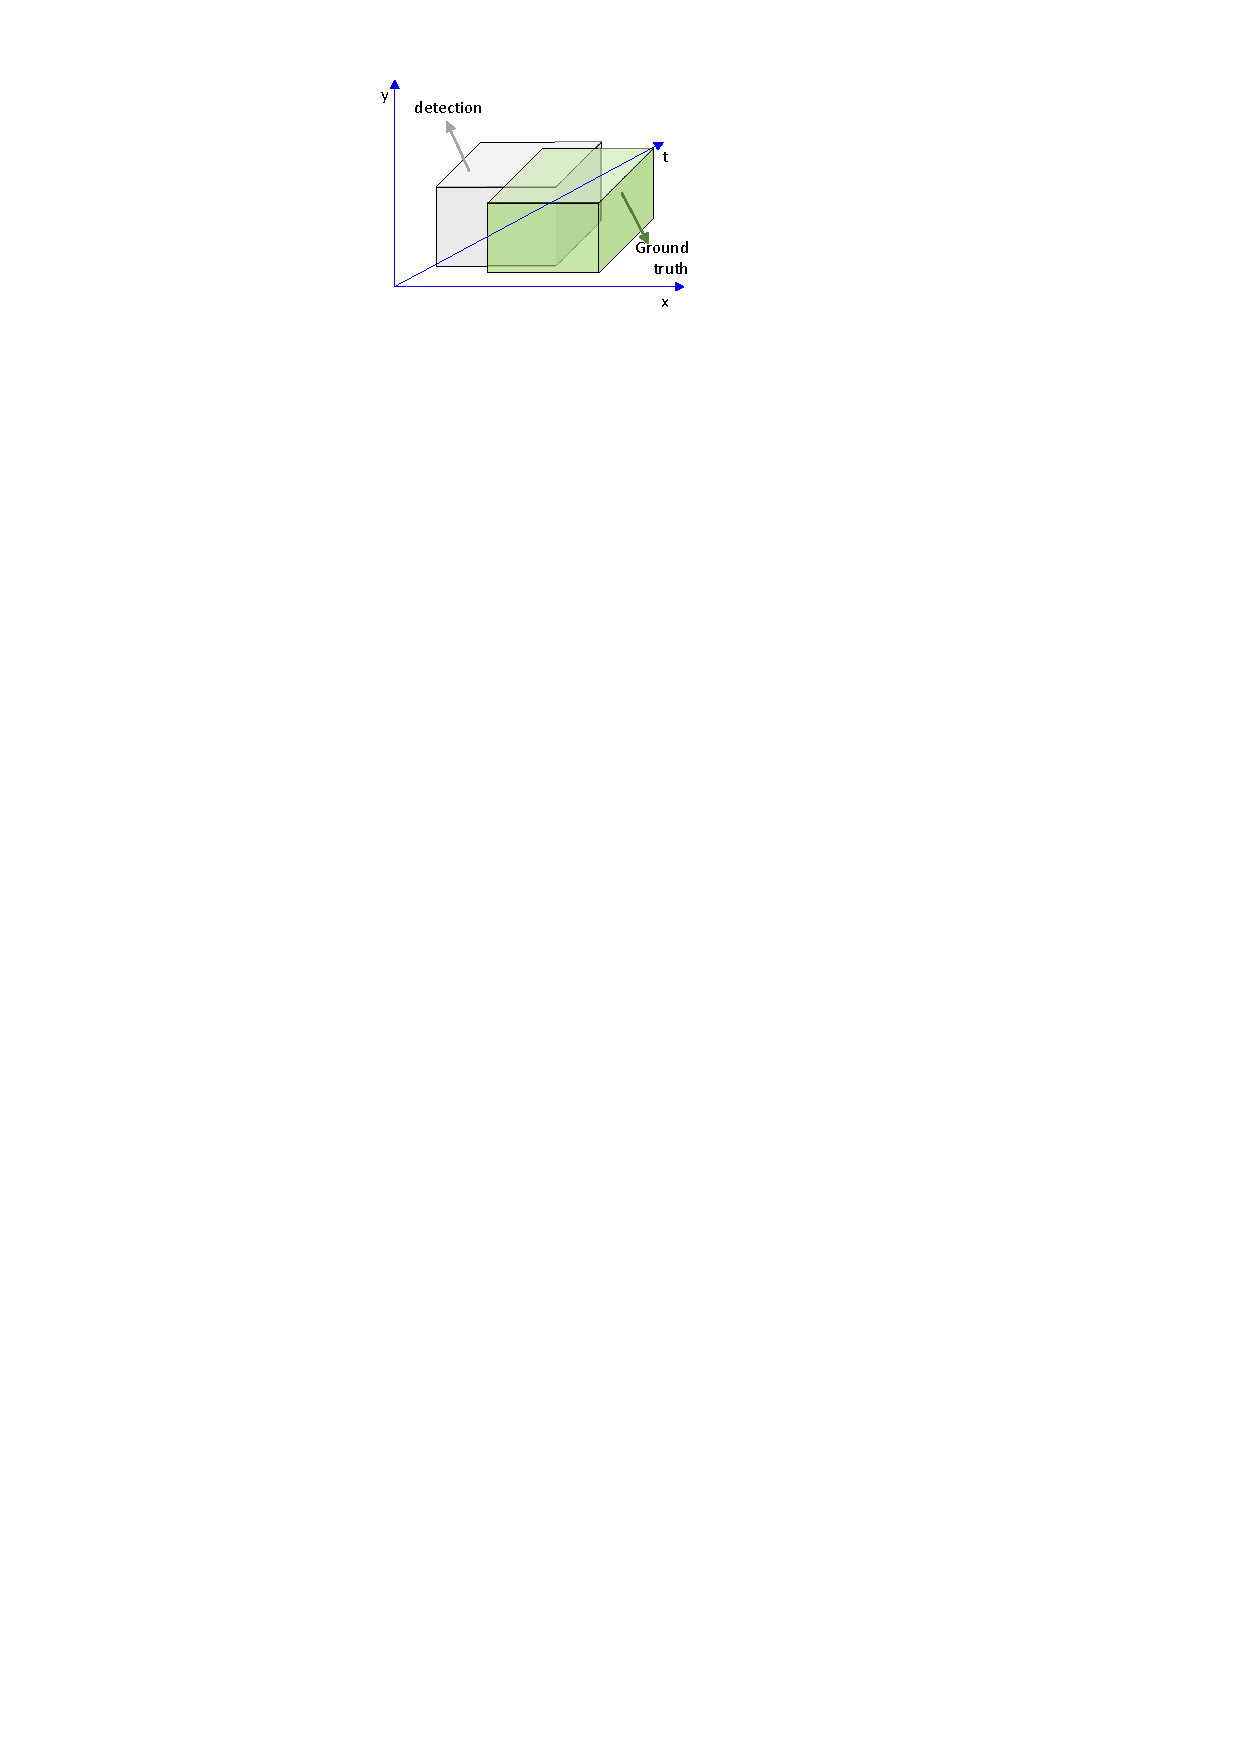
\includegraphics[trim=2cm 24.7cm 0cm 1cm]{figs/ut_det.pdf}
	\caption{Illustration of detection and ground truth.  }
	\label{fig:ut_det}
\end{figure}
\par 
We use general Precision-Recall graph to evaluate our detection model. Where precision and recall are defined as below:
\begin{equation*}
\text{Precision} = \frac{\text{The number of correct detections}}{\text{The number of founded detections}}
\end{equation*}

\begin{equation*}
\text{Recall} = \frac{\text{The number of correct detections}}{\text{The number of GT detections}}
\end{equation*}

\subsubsection*{The challenges} 
Comparing with image analysis focus on still images, we are expected to recognize ongoing complex human activities from continuous videos, taken in realistic settings. There are some challenges for the classification task as below:
\begin{enumerate}
	\item The backgrounds of set1 and set2 are different illustrated in Figure \ref{fig:ut_challenges_1} a). This requires the classifier focuses on foregrounds and ignore the influences of different backgrounds. 
	\item The background is not still even in a same video segment which is illustrated in Figure \ref{fig:ut_challenges_1} b). This may causes troubles for the classifier to learn to discriminate between the background and the foreground.    
	\item The resolutions of different video segments are different which is illustrated in Figure \ref{fig:ut_challenges_1} c). The classifier usually requires all its inputs with the unified size. we can unify the sizes for them by cropping and resizing. But, the width-height ratio and scale for each interaction may still be different. 
	\item The time duration for each interaction execution in different video segments varies much from 30 frames to 154 frames.
	\item The lighting conditions of different video segments are various which is illustrated in Figure \ref{fig:ut_challenges_1} d).  
\end{enumerate} 
\begin{figure}
	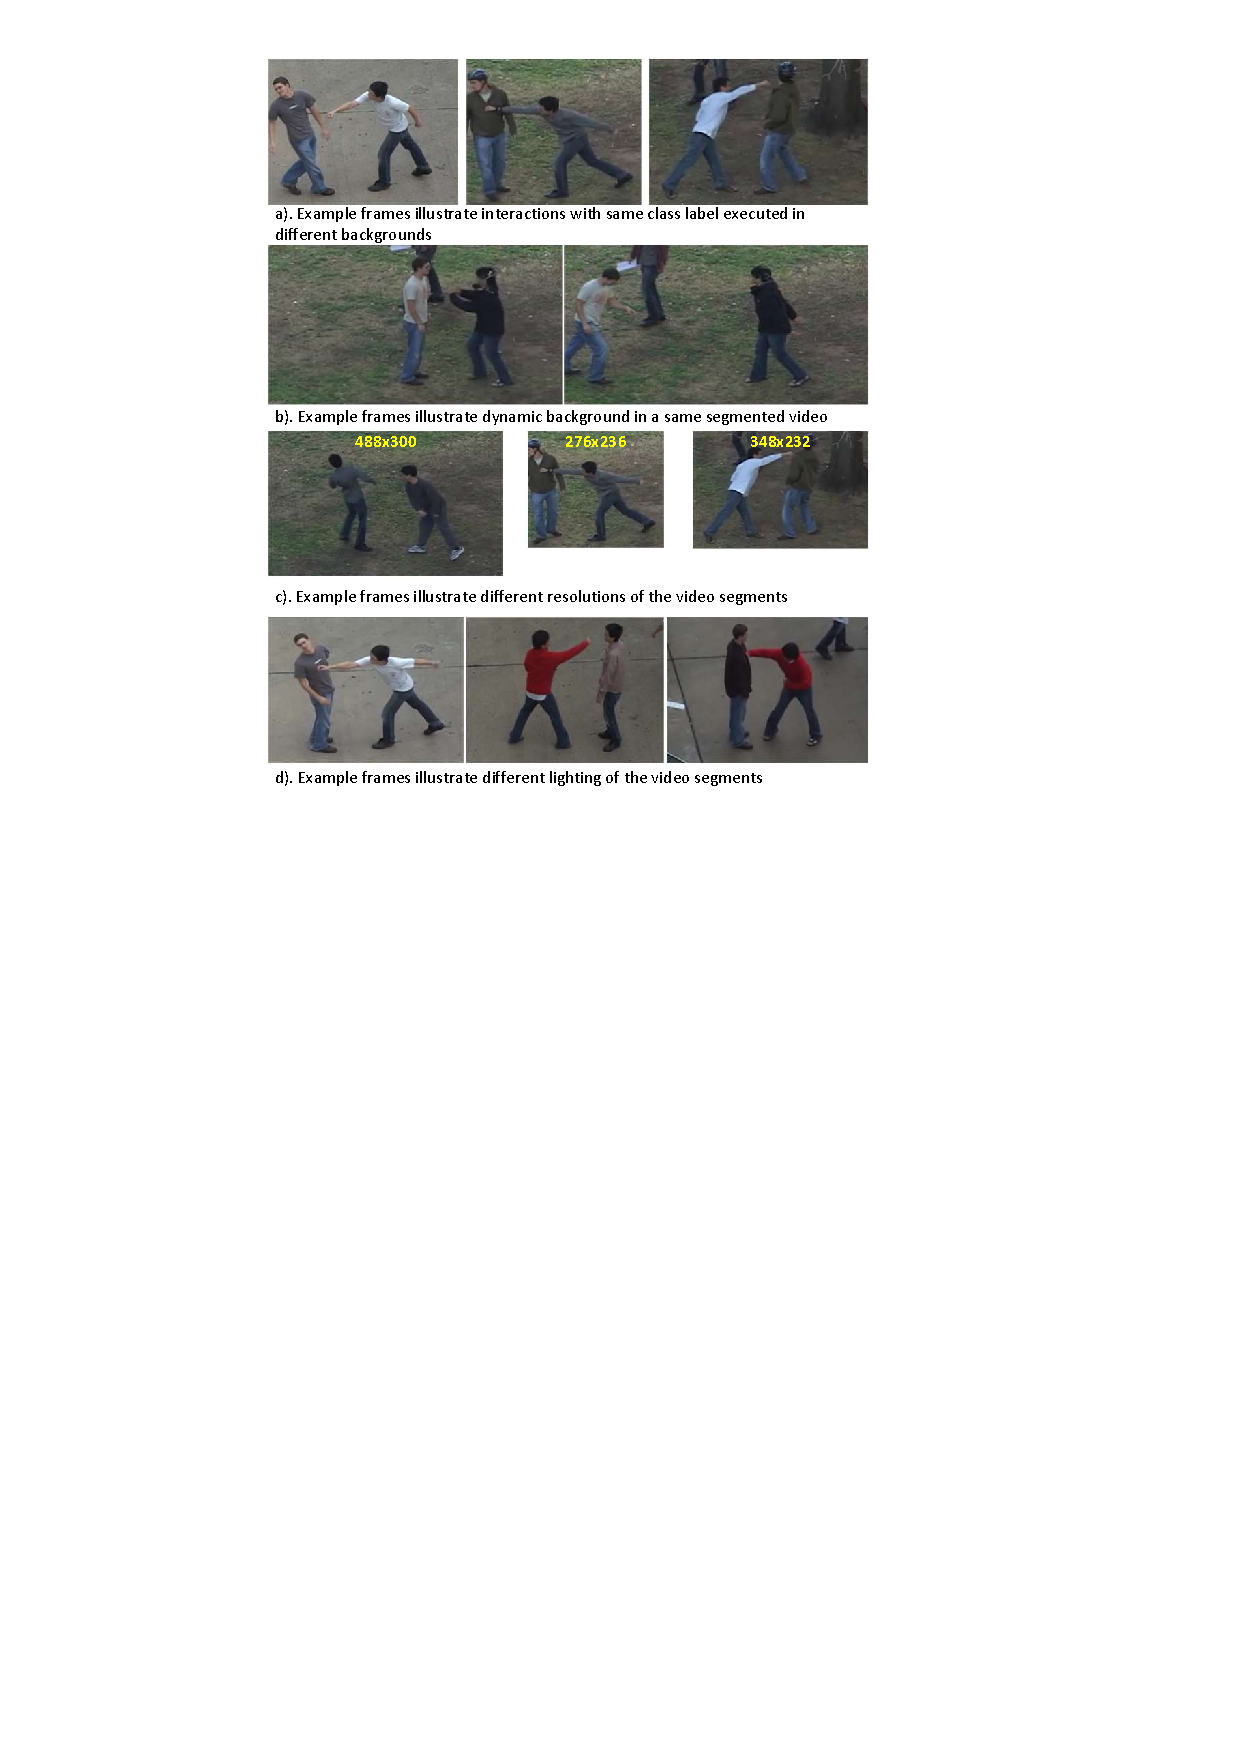
\includegraphics[trim=2cm 16.5cm 0cm 1cm]{figs/ut_challenges_1.pdf}
	\caption{Some challenges for the classification task. }
	\label{fig:ut_challenges_1}
\end{figure}

Compared with the classification task, there are some extra challenges for the detection task, including:
\begin{enumerate}
	\item Both interacting people and irrelevant people are present in the scene in some videos as shown in Figure \ref{fig:ut_challenges_2} a). This will causes troubles for interacting people detection.
	\item Several pairs of interacting people execute interactions simultaneously in some videos as shown in Figure \ref{fig:ut_challenges_2} b), but the ground truth only contains one pair interacting people for each video. 
\end{enumerate}
\begin{figure}
	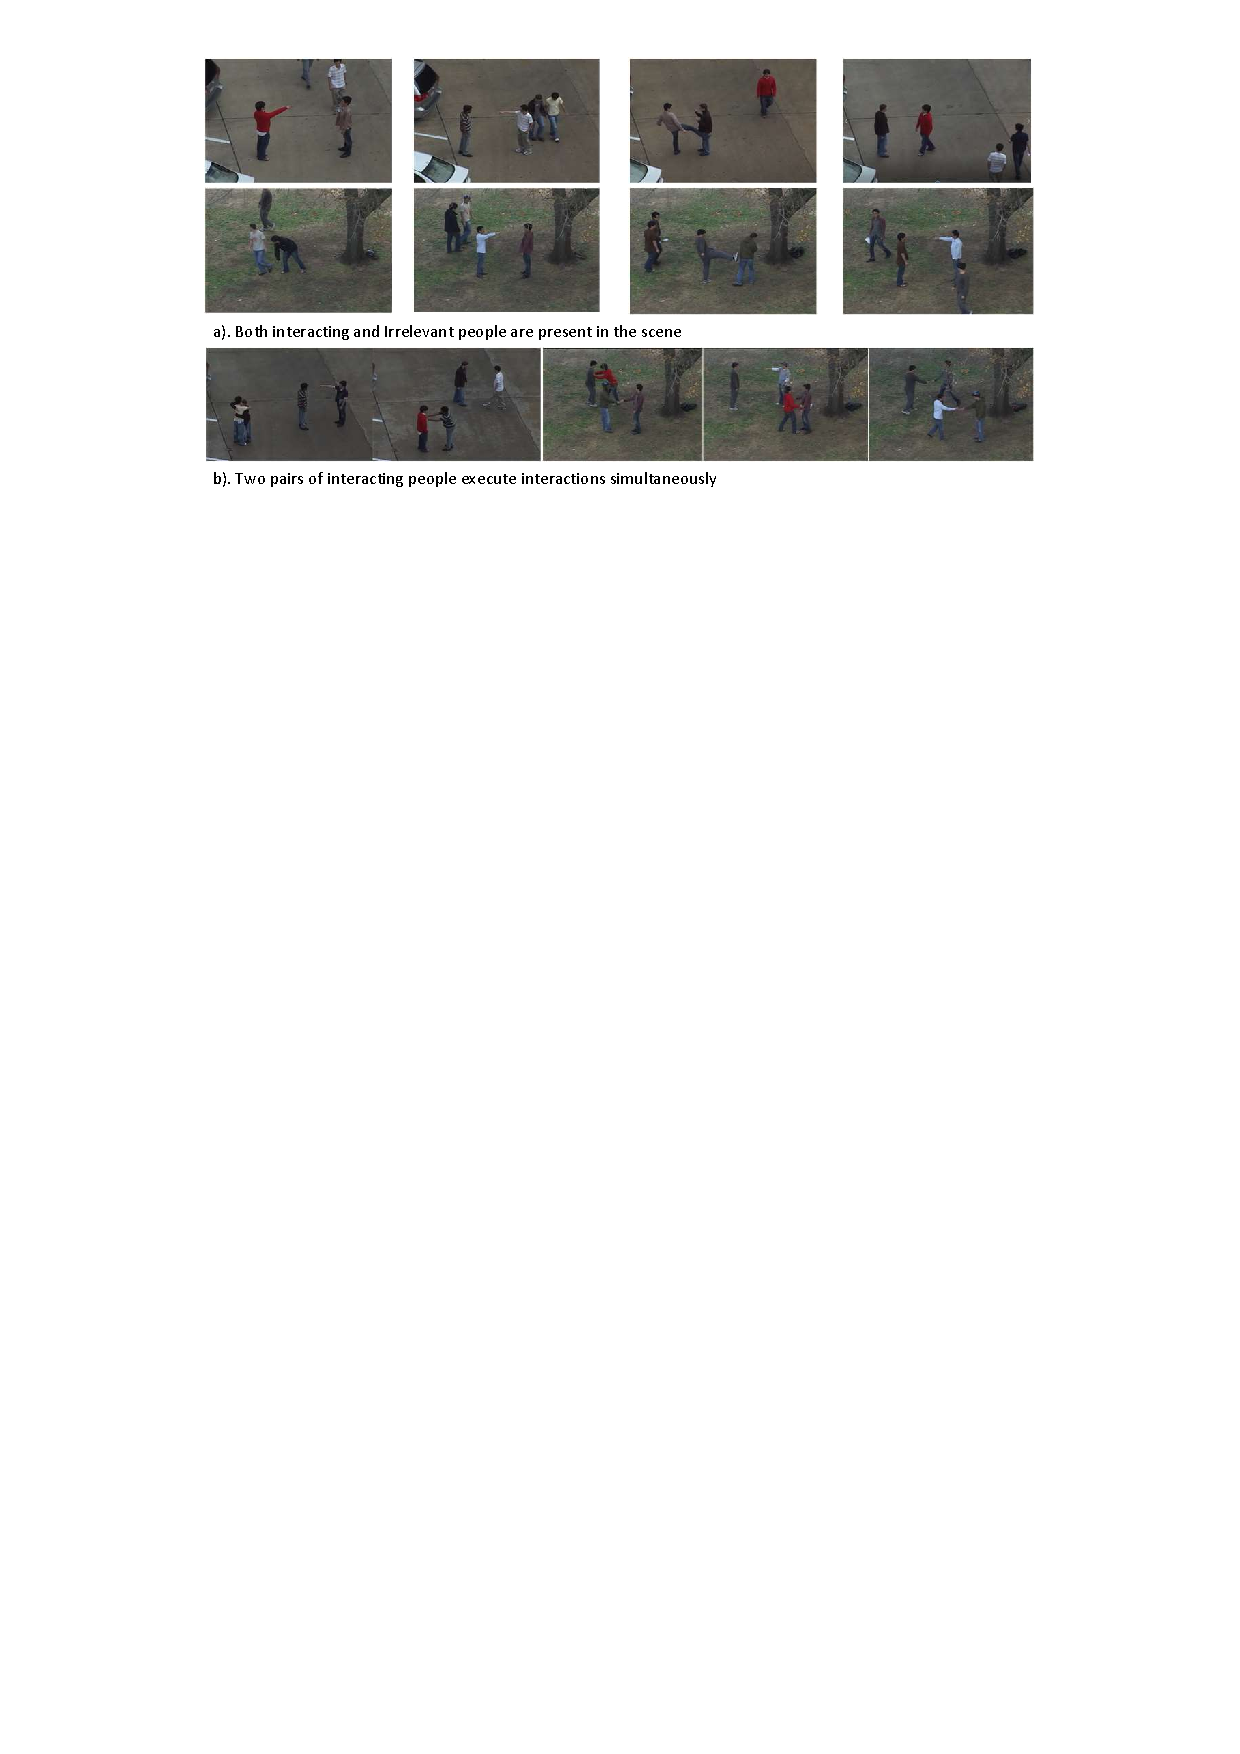
\includegraphics[trim=2cm 21.5cm 0cm 1cm]{figs/ut_challenges_2.pdf}
	\caption{Illustrations of some extra challenges for the detection task. }
	\label{fig:ut_challenges_2}
\end{figure}
%=========================================================